\chapter{Applications} %\seb{$\checkmark$} }
\label{ch:appl}

%\epigraph{
%Earth's crammed with heaven, \\
%And every common bush afire with God, \\
%But only he who sees takes off his shoes; \\
%The rest sit round and pluck blackberries.
%}
%{\textsc{Elizabeth Barrett Browning}}


Theorem~\ref{thm:weakconv} gives verifiable conditions under which interacting particle systems with dynamics in the form of Algorithm~\ref{alg:SMC} have asymptotically Kingman genealogies. 
The work was motivated by SMC algorithms, which have the required form. However, certain choices of state space and dynamics within the context of Algorithm~\ref{alg:SMC} yield systems that are not very SMC-like but may have applications in other fields such as population genetics. 
For instance, we have generally imagined that the resampling scheme is unbiased, but this is by no means necessary for Theorem~\ref{thm:weakconv} (or indeed Theorem~\ref{thm:FDDconv}); it is just that biased resampling schemes are of little use in SMC.

The applications presented in this chapter are all motivated by SMC, but an interesting area of future research would be to explore the implications of Theorem~\ref{thm:weakconv} in other contexts. From the population genetics point-of-view, Theorem~\ref{thm:weakconv} may be seen as a complement to the convergence criteria for neutral models discussed in Section \ref{sec:previousgeneconv}, so it would be interesting to construct some corollaries for classical non-neutral population models.

For many of the following results it will be necessary to compute filtered expectations $\Et[\cdot]$, which are generally difficult to compute directly. 
To simplify the computations we introduce a sequence of $\sigma$-algebras $(\mathcal{H}_t)$, defined below, such that filtered expectations can be written in terms of conditional expectations given $\mathcal{H}_t$.

Figure \ref{fig:cond_indep_graph_Ht} shows a section of the conditional dependence graph implied by Algorithm \ref{alg:SMC}, as in Figure~\ref{fig:cond_indep_graph}, except that time is now labelled in reverse. The $\sigma$-algebra
\begin{equation}\label{eq:defn_Ht}
\mathcal{H}_t := \sigma(X_{t-1}^{(1:N)}, X_t^{(1:N)}, w_{t-1}^{(1:N)}, w_t^{(1:N)} ) ,
\end{equation}
at each time $t$, forms a separatrix (in the sense of d-separation; see \textcite{verma1988}) between the parental indices $a_t^{(1:N)}$ and the previous $\sigma$-algebra $\mathcal{F}_{t-1}$ in the filtration. 
That is, $a_t^{(1:N)}$ is conditionally independent of $\mathcal{F}_{t-1}$ given $\mathcal{H}_t$.
The practical upshot of this is that we can use the tower rule along with conditional independence to write filtered expectations as
\begin{equation}
\Et[ f(\nu_t^{(1:N)}) ] 
= \Et\left[ \E[ f(\nu_t^{(1:N)}) \mid \mathcal{H}_t, \mathcal{F}_{t-1} ] \right] 
= \Et\left[ \E[ f(\nu_t^{(1:N)}) \mid \mathcal{H}_t ] \right] . \label{eq:condexp_HtFt}
\end{equation}
As we will see, this enables us to compute bounds on the filtered expectations of interest relatively easily.

\begin{figure}[ht]
\centering
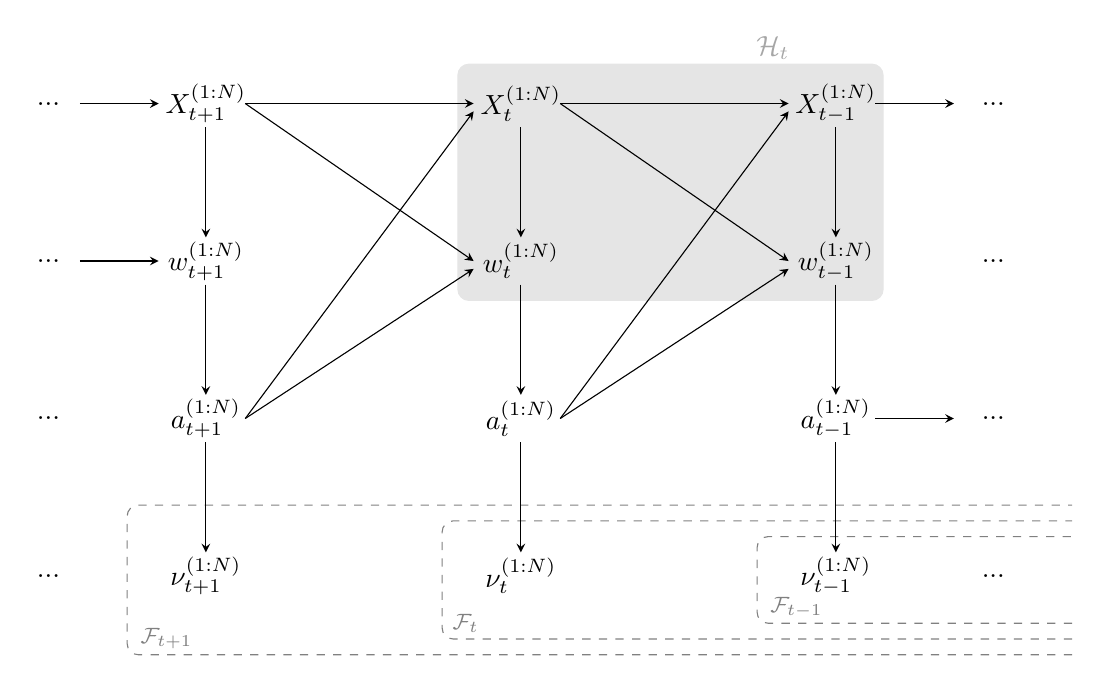
\begin{tikzpicture}[>=stealth]
% separatrix
\filldraw[gray!20, rounded corners] (3.2,0.5)--(8.6,0.5)--(8.6,-2.5)--(3.2,-2.5)--cycle;
\node[gray!70] at (7.2,0.7) {$\mathcal{H}_t$};
% left dots
\node at (-2,0) {...};
\node at (-2,-2) {...};
\node at (-2,-4) {...};
\node at (-2,-6) {...};
% labels (t+1)
\node at (0,0) {$X_{t+1}^{(1:N)}$};
\node at (0,-2) {$w_{t+1}^{(1:N)}$};
\node at (0,-4) {$a_{t+1}^{(1:N)}$};
\node at (0,-6) {$\nu_{t+1}^{(1:N)}$};
% labels t
\node at (4,0) {$X_{t}^{(1:N)}$};
\node at (4,-2) {$w_{t}^{(1:N)}$};
\node at (4,-4) {$a_{t}^{(1:N)}$};
\node at (4,-6) {$\nu_{t}^{(1:N)}$};
% labels (t-1)
\node at (8,0) {$X_{t-1}^{(1:N)}$};
\node at (8,-2) {$w_{t-1}^{(1:N)}$};
\node at (8,-4) {$a_{t-1}^{(1:N)}$};
\node at (8,-6) {$\nu_{t-1}^{(1:N)}$};
% right dots
\node at (10,0) {...};
\node at (10,-2) {...};
\node at (10,-4) {...};
\node at (10,-6) {...};
%filtrations
\draw [rounded corners, dashed, gray] (11,-6.6)--(7,-6.6)--(7,-5.5)--(11,-5.5);
\draw [rounded corners, dashed, gray] (11,-6.8)--(3,-6.8)--(3,-5.3)--(11,-5.3);
\draw [rounded corners, dashed, gray] (11,-7)--(-1,-7)--(-1,-5.1)--(11,-5.1);
% filtration labels
\node[gray] at (7.5,-6.4) {\footnotesize{$\mathcal{F}_{t-1}$}};
\node[gray] at (3.3,-6.6) {\footnotesize{$\mathcal{F}_{t}$}};
\node[gray] at (-0.5,-6.8) {\footnotesize{$\mathcal{F}_{t+1}$}};
% arrows (t+1) -> t
\draw[->] (0.5,0)--(3.4,0);
\draw[->] (0.5,0)--(3.4,-2);
\draw[->] (0.5,-4)--(3.4,-2.1);
\draw[->] (0.5,-4)--(3.4,-0.1);
% arrows t -> (t-1)
\draw[->] (4.5,0)--(7.4,0);
\draw[->] (4.5,0)--(7.4,-2);
\draw[->] (4.5,-4)--(7.4,-2.1);
\draw[->] (4.5,-4)--(7.4,-0.1);
% vertical arrows (t+1)
\draw[->] (0,-0.3)--(0,-1.7);
\draw[->] (0,-2.3)--(0,-3.7);
\draw[->] (0,-4.3)--(0,-5.7);
% vertical arrows t
\draw[->] (4,-0.3)--(4,-1.7);
\draw[->] (4,-2.3)--(4,-3.7);
\draw[->] (4,-4.3)--(4,-5.7);
% vertical arrows (t-1)
\draw[->] (8,-0.3)--(8,-1.7);
\draw[->] (8,-2.3)--(8,-3.7);
\draw[->] (8,-4.3)--(8,-5.7);
% arrows ... -> t+1
\draw[->] (-1.6,0)--(-0.6,0);
\draw[->] (-1.6,-2)--(-0.6,-2);
% arrows t-1 -> ...
\draw[->] (8.5,0)--(9.5,0);
\draw[->] (8.5,-4)--(9.5,-4);
\end{tikzpicture}
\caption[Construction of separatrix $\mathcal{H}_t$]{Part of the conditional dependence graph implied by Algorithm \ref{alg:SMC} illustrating the construction of $\mathcal{H}_t$. The direction of time is from left to right. The reverse-time filtration is indicated by the dashed areas. The nodes highlighted in grey generate the separatrix $\mathcal{H}_t$ between $a_t^{(1:N)}$ and $\mathcal{F}_{t-1}$.}
\label{fig:cond_indep_graph_Ht}
\end{figure}




\section{Multinomial resampling}
\label{sec:corol_mn}
Multinomial resampling is often preferred in theoretical studies of SMC, because it renders the parental indices conditionally i.i.d. given the weights, making it relatively simple to analyse the resulting algorithm.
The convergence of finite-dimensional distributions for multinomial resampling was proved in \textcite[Corollary 1]{koskela2018}, but we are now able to prove an analogous weak convergence result. The following proof also demonstrates the relative ease with which we can verify Theorem~\ref{thm:FDDconv} as opposed to \textcite[Theorem 1]{koskela2018}.
%The result of Corollary~\ref{thm:multinomial} was proved in \textcite[Corollary 1]{koskela2018}. It is also included here, firstly to demonstrate the relative ease with which it is proved under Theorem~\ref{thm:FDDconv} as opposed to \textcite[Theorem 1]{koskela2018}, and secondly to introduce the proof technique before proceeding to more complex resampling schemes.

\begin{corollary}\label{thm:multinomial}
Consider an SMC algorithm using multinomial resampling, such that \ref{standing_assumption} is satisfied. Assume there exist constants $\varepsilon\in (0,1], a\in [1,\infty)$ and probability density $h$ such that for all $x, x^\prime, t$,
\begin{equation}\label{eq:gq_bounds_mn}
\frac{1}{a} \leq g_t(x, x^\prime) \leq a , \quad
\varepsilon h(x^\prime) \leq q_t(x, x^\prime) \leq \frac{1}{\varepsilon} h(x^\prime) .
\end{equation}
Let $(G_t^{(n,N)})_{t\geq0}$ denote the genealogy of a random sample of $n$ terminal particles from the output of the algorithm among a total of $N$ particles. Then, for any fixed $n$, the time-scaled genealogy $(G_{\tau_N(t)}^{(n,N)})_{t\geq0}$ converges weakly to Kingman's $n$-coalescent as $N\to \infty$.%, in the sense of finite-dimensional distributions.
\end{corollary}
The bounds on $g_t$ and $q_t$ in \eqref{eq:gq_bounds_mn} are rather strong; they can only reasonably be expected to hold if the state space is compact. 
However, they are widespread in the literature, where they are known as the \emph{strong mixing conditions} \parencite[Section 3.5.2]{delmoral2004}, because they greatly facilitate the theoretical analysis of SMC algorithms. It is often possible to relax these conditions at the expense of considerable technical complication.
The conditions on $g_t$ in \eqref{eq:gq_bounds_mn} ensure that the weights are all $O(N^{-1})$, none of them being too close to zero or one. Together with the bounds on $q_t$, this is enough to control the relative rate of multiple mergers, as seen in the following proof.
%In the following proof, conditions \eqref{eq:gq_bounds_mn} ensure that the weights are all $O(N^{-1})$, none of them being too close to zero or one, which controls the relative rate of multiple mergers.

\begin{proof}
%Define the $\sigma$-algebras $\mathcal{H}_t$ as in \eqref{eq:defn_Ht}.
%Recall that the sequence of $\sigma$-algebras
%\begin{equation}%\label{eq:defn_Ht}
%\mathcal{H}_t := \sigma(X_{t-1}^{(1:N)}, X_t^{(1:N)}, w_{t-1}^{(1:N)}, w_t^{(1:N)} )
%\end{equation}
%are such that $\nu_t^{(1:N)}$ is conditionally independent of the filtration $\mathcal{F}_{t-1}$ given $\mathcal{H}_t$.
Define $\mathcal{H}_t$ as in \eqref{eq:defn_Ht}.
Conditional on $\mathcal{H}_t$ the parental indices are independent, with conditional law
\begin{equation}\label{eq:parentslaw_mn}
\Prob \left[ a_t^{(i)} = a_i \mid \mathcal{H}_t \right] 
%\propto w_t^{(a_i)} q_{t-1}(X_t^{(a_i)}, X_{t-1}^{(i)})
\propto g_t( X_{t+1}^{a_{t+1}^{(a_i)}} , X_t^{(a_i)} ) q_{t-1}(X_t^{(a_i)}, X_{t-1}^{(i)})
\end{equation}
for each $i$, so the joint law is
\begin{equation*}
\Prob \left[ a_t^{(1:N)} = a_{1:N} \mid \mathcal{H}_t \right] 
%\propto \prod_{i=1}^N w_t^{(a_i)} q_{t-1}(X_t^{(a_i)}, X_{t-1}^{(i)}).
\propto \prod_{i=1}^N g_t( X_{t+1}^{a_{t+1}^{(a_i)}} , X_t^{(a_i)} ) 
        q_{t-1}(X_t^{(a_i)}, X_{t-1}^{(i)}).
\end{equation*}
%
%%%%%%%%%
%
%The bounds on $g_t$ in \eqref{eq:gq_bounds_mn} imply 
%almost sure bounds on the weights
%%the almost sure bounds
%%\begin{equation*}
%%\frac{1}{a^2 N}
%%\leq w_t^{(i)}
%%\leq \frac{a^2}{N}
%%\end{equation*}
%which, along with the bounds on $q_{t-1}$ from \eqref{eq:gq_bounds_mn}, allows us to apply a balls-in-bins coupling presented in \textcite[Proof of Lemma 3]{koskela2018} to obtain bounds on expectations of functions of $a_t^{(1:N)}$.
Using the bounds \eqref{eq:gq_bounds_mn} and the balls-in-bins coupling of \textcite[Proof of Lemma 3]{koskela2018}, we can obtain bounds on expectations of functions of $a_t^{(1:N)}$.
For any $k\in\mathbb{N}$ the function $a_t^{(1:N)} \to (\nu_t^{(i)})_k$ is $\{i\}$-increasing in the sense of \textcite{koskela2018}, so we may apply the bounds
\begin{equation*}
\E[ (V_1^{(i)})_k ]
\leq \E[ (\nu_t^{(i)})_k \mid \mathcal{H}_t ]
\leq \E[ (V_2^{(i)})_k ] ,
\end{equation*}
where
\begin{align*}
& V_1^{(i)} 
\sim \Bin\left(N, \frac{\varepsilon/a}{(\varepsilon/a) + (N-1)(a/\varepsilon)} \right),\\
& V_2^{(i)} 
\sim \Bin\left( N, \frac{a/\varepsilon}{(a/\varepsilon) + (N-1)(\varepsilon/a)} \right) .
\end{align*}
independently for each $i$ and independently of $\mathcal{F}_\infty$.
Furthermore, using the moments of the Binomial distribution \parencite[see for example][p. 67]{mosimann1962}
\begin{equation*}
\E[ (V_1^{(i)})_k ]
= (N)_k \left( \frac{ \varepsilon/a }{ (\varepsilon/a) + (N-1)(a/\varepsilon) } \right)^k
\geq (N)_k \left( \frac{ \varepsilon/a }{ N(a/\varepsilon) } \right)^k
= \frac{(N)_k}{N^k} \frac{\varepsilon^{2k}}{a^{2k}} .
\end{equation*}
Similarly, 
\begin{equation*}
\E[ (V_2^{(i)})_k ]
\leq \frac{(N)_k}{N^k} \frac{a^{2k}}{\varepsilon^{2k}} .
\end{equation*}
We therefore have the bounds
\begin{equation*}
\frac{(N)_k}{N^k} \frac{\varepsilon^{2k}}{a^{2k}}
\leq \E[ (\nu_t^{(i)})_k \mid \mathcal{H}_t ]
\leq \frac{(N)_k}{N^k} \frac{a^{2k}}{\varepsilon^{2k}} . %\label{eq:mn_nuk_bounds}
\end{equation*}
for each $k$. Consequently,
\begin{equation}
\frac{1}{(N)_2} \sum_{i=1}^N \E[ (\nu_t^{(i)})_2 \mid \mathcal{H}_t ]
\geq \frac{\varepsilon^4}{Na^4} \label{eq:mn_cN_LB}
\end{equation}
and
\begin{equation}
\frac{1}{(N)_3} \sum_{i=1}^N \E[ (\nu_t^{(i)})_3 \mid \mathcal{H}_t ]
\leq \frac{a^6}{N^2 \varepsilon^6} . \label{eq:mn_cN3_UB}
\end{equation}
%
%%%%%%%%%
%
%\textcite{koskela2018} makes the following observation, which follows from a balls-in-bins coupling.
%Assume \eqref{eq:gq_bounds_mn}. 
%Then for any function $f:\{1,\dots,N\}^N \to \mathbb{R}$ such that (for a fixed $i$) $f(a_t^{\prime(1:N)}) \geq f(a_t^{(1:N)})$ whenever $|\{j:a_t^{\prime(j)}=i\}| \geq |\{j:a_t^{(j)}=i\}|$,
%\begin{equation}\label{eq:mn_f_bound}
%\E[ f(A_{1,i}^{(1:N)}) ] 
%\leq \E[ f(a_t^{(1:N)}) \mid \mathcal{H}_t ]
%\leq \E[ f(A_{2,i}^{(1:N)}) ] 
%\end{equation}
%where the elements of $A_{1,i}^{(1:N)}, A_{2,i}^{(1:N)}$ are all mutually independent and independent of $\mathcal{F}_{\infty}$, and distributed according to
%\begin{align*}
%& A_{1,i}^{(j)} 
%\sim \Cat \left( (\varepsilon/a)^{\1{i=1} -\1{i\neq 1}} ,
%        \dots, (\varepsilon/a)^{\1{i=N} -\1{i\neq N}} \right) \\
%& A_{2,i}^{(j)} 
%\sim \Cat \left( (a/\varepsilon)^{\1{i=1} -\1{i\neq 1}} ,
%        \dots, (a/\varepsilon)^{\1{i=N} -\1{i\neq N}} \right)
%\end{align*}
%independently for each $j$, where the vector of probabilities is given up to a constant in the argument of Categorical distributions.
%We will use these random vectors to construct bounds that are independent of $\mathcal{F}_\infty$.
%Also define the corresponding offspring counts $V_1^{(i)} = |\{j: A_{1,i}^{(j)}=i\}|$, $V_2^{(i)} = |\{j: A_{2,i}^{(j)}=i\}|$, for $i=1,\dots,N$, which have marginal distributions
%\begin{align*}
%& V_1^{(i)} 
%\sim \Bin\left(N, \frac{\varepsilon/a}{(\varepsilon/a) + (N-1)(a/\varepsilon)} \right),\\
%& V_2^{(i)} 
%\sim \Bin\left( N, \frac{a/\varepsilon}{(a/\varepsilon) + (N-1)(\varepsilon/a)} \right) .
%\end{align*}
%\seb{ Could state that a particular consequence of \eqref{eq:mn_f_bound} and $V_1,V_2$ etc.\ is
%\begin{equation*}
%\frac{(N)_k}{N^k} \frac{\varepsilon^{2k}}{a^{2k}}
%\leq \E[ (\nu_t^{(i)})_k \mid \mathcal{H}_t ]
%\leq \frac{(N)_k}{N^k} \frac{a^{2k}}{\varepsilon^{2k}} .
%\end{equation*}
%for any $k\in\mathbb{N}$? This is easily proved in much the same way as the two special cases below. This could probably replace \eqref{eq:mn_f_bound} and the surrounding argument, since all $f$s we use are of this particular form.}
%Now consider the function $f_i(a_t^{(1:N)}) := (\nu_t^{(i)})_2$. We can apply \eqref{eq:mn_f_bound} to obtain the lower bound
%\begin{align}
%\frac{1}{(N)_2} \sum_{i=1}^N \E[ (\nu_t^{(i)})_2 \mid \mathcal{H}_t ]
%&\geq \frac{1}{(N)_2} \sum_{i=1}^N \E[ (V_1^{(i)})_2 ]
%= \frac{1}{(N)_2} \sum_{i=1}^N (N)_2 \left[ \frac{ \varepsilon/a}{ (\varepsilon/a) + (N-1)(a/\varepsilon) } \right]^2 \notag\\
%&\geq \sum_{i=1}^N \left[ \frac{ \varepsilon/a}{ N a/\varepsilon } \right]^2
%= \frac{\varepsilon^4}{Na^4} \label{eq:mn_cN_LB}
%\end{align}
%using the moments of the Binomial distribution \parencite[see for example]{mosimann1962}.
%Similarly, we derive an upper bound on $f_i(a_t^{(1:N)}) := (\nu_t^{(i)})_3$:
%\begin{align}
%\frac{1}{(N)_3} \sum_{i=1}^N \E[ (\nu_t^{(i)})_3 \mid \mathcal{H}_t]
%&\leq \frac{1}{(N)_3} \left[ \sum_{i=1}^N \E[ (V_2^{(i)})_3 ] \right]
%= \frac{1}{(N)_3} \sum_{i=1}^N (N)_3 \left[ \frac{ a/\varepsilon }{ (a/\varepsilon) + (N-1)(\varepsilon/a) } \right]^3 \notag\\
%&\leq \sum_{i=1}^N \left[ \frac{ a/\varepsilon }{ N \varepsilon/a } \right]^3
%= \frac{a^6}{N^2\varepsilon^6} . \label{eq:mn_cN3_UB}
%\end{align}
%
%The definition of $\mathcal{H}_t$ is such that, for any suitable function $f$, by the tower property and conditional independence we have
%\begin{equation}
%\Et[ f(\nu_t^{(1:N)}) ] 
%= \Et\left[ \E[ f(\nu_t^{(1:N)}) \mid \mathcal{H}_t, \mathcal{F}_{t-1} ] \right] 
%= \Et\left[ \E[ f(\nu_t^{(1:N)}) \mid \mathcal{H}_t ] \right] .\label{eq:condexp_HtFt}
%\end{equation}
Applying \eqref{eq:condexp_HtFt} to \eqref{eq:mn_cN_LB} and \eqref{eq:mn_cN3_UB} we find
\begin{align*}
\frac{\frac{1}{(N)_3} \sum_{i=1}^N \Et[ (\nu_t^{(i)})_3 ]}{\frac{1}{(N)_2} \sum_{i=1}^N \Et[ (\nu_t^{(i)})_2 ]}
&\leq \frac{ a^6 / (N^2 \varepsilon^6) }{ \varepsilon^4 / (N a^4) }
= \frac{ a^{10} }{ N\varepsilon^{10} }
=: b_N \underset{N\to\infty}{\longrightarrow} 0.
\end{align*}
Thus \eqref{eq:mainthmcond} is satisfied. 
It remains to show that, for $N$ sufficiently large, $\Prob[ \tau_N(t) = \infty ] =0$ for all finite $t$, a technicality which is proved in Lemma \ref{thm:mn_nontriviality}. 
Applying Theorem~\ref{thm:weakconv} then yields the result.
\end{proof}



\begin{lemma}\label{thm:mn_nontriviality}
Consider an SMC algorithm using multinomial resampling, satisfying \ref{standing_assumption} and \eqref{eq:gq_bounds_mn}. 
Then, for all $N>2$, $\Prob[ \tau_N(t) = \infty ]=0$ for all finite $t$.
\end{lemma}

\begin{proof}
Since $c_N(t) \in [0,1]$ almost surely and has strictly positive expectation, for any fixed $N$ the distribution of $c_N(t)$ with given expectation that maximises $\Prob[ c_N(t)=0 \mid \mathcal{F}_{t-1} ]$ is two atoms, at 0 and 1 respectively. To ensure the correct expectation, the atom at 1 should have mass $\Prob[ c_N(t)=1 \mid \mathcal{F}_{t-1} ] = \Et [ c_N(t) ]$, which is bounded below by \eqref{eq:mn_cN_LB}.
If $c_N(t) > 0$ then $c_N(t) \geq 2/(N)_2 > 2/N^2$. Hence, in general $\Prob[ c_N(t) > 2/N^2 \mid \mathcal{F}_{t-1} ] \geq \Et [c_N(t)]$. 
Applying \eqref{eq:mn_cN_LB} along with \eqref{eq:condexp_HtFt}, we have for any finite $N$
\begin{equation*}
\sum_{t=0}^\infty \Prob[ c_N(t) > 2/N^2 \mid \mathcal{F}_{t-1} ]
\geq \sum_{t=0}^\infty \Et [ c_N(t) ]
\geq \sum_{t=0}^\infty \frac{\varepsilon^4}{Na^4}
= \infty .
\end{equation*}
By a filtered version of the second Borel--Cantelli lemma \parencite[see for example][Theorem 4.3.4]{durrett2019}, this implies that $c_N(t) >2/N^2$ for infinitely many $t$, almost surely.
This ensures, for all $t <\infty$, that $\Prob\left[ \exists s<\infty : \sum_{r=1}^s c_N(r) \geq t \right] =1$, which by definition of $\tau_N(t)$ is equivalent to $\Prob[ \tau_N(t) = \infty ] =0$.
\end{proof}




\section{Stratified resampling}

\begin{corollary}\label{thm:stratified}
Consider an SMC algorithm using stratified resampling, such that \ref{standing_assumption} is satisfied.
Assume that there exists a constant $a\in [1,\infty)$ such that for all $x, x^\prime, t$,
\begin{equation}\label{eq:gq_bounds_sr}
\frac{1}{a} \leq g_t(x, x^\prime) \leq a .
\end{equation}
Assume that $\Prob[ \tau_N(t) = \infty] =0$ for all finite $t$.
Let $(G_t^{(n,N)})_{t\geq0}$ denote the genealogy of a random sample of $n$ terminal particles from the output of the algorithm among a total of $N$ particles. Then, for any fixed $n$, the time-scaled genealogy $(G_{\tau_N(t)}^{(n,N)})_{t\geq0}$ converges weakly to Kingman's $n$-coalescent as $N\to \infty$.%, in the sense of finite-dimensional distributions.
\end{corollary}
Stratified resampling is, by design, much more restrictive than multinomial resampling. Once the weights are known there is little freedom in the offspring counts, so it is not surprising that control over the weights such as \eqref{eq:gq_bounds_sr} provides is sufficient without any additional control over the transition densities $q_t$. 
Indeed the transition kernels need not even admit densities.
This is in contrast to multinomial resampling (Corollary~\ref{thm:multinomial}), where $g_t$ and $q_t$ are more or less on an equal footing, and we require both to be bounded.

It is not immediately clear that the finite time scale condition $\Prob[ \tau_N(t) = \infty] =0$ holds under conditions \eqref{eq:gq_bounds_sr}, so it is included in the statement of the corollary. Proposition~\ref{thm:SR_nontriviality} presents some sufficient conditions for the finite time scale, but these are by no means necessary.

\begin{proof}
Define the $\sigma$-algebras $\mathcal{H}_t$ as in \eqref{eq:defn_Ht}.
With stratified resampling, conditional on the weights each offspring count almost surely takes one of four values: $\nu_t^{(i)} \in \{ \flnw -1, \flnw, \flnw +1, \flnw +2 \}$.  
Define for each $k\in\mathbb{Z}$
\begin{equation}\label{eq:pk_defn}
p_k^{(i)} := \Prob \left[ \nu_t^{(i)} = \flnw + k \midd \mathcal{H}_t \right] .
\end{equation}
Then $p_k^{(i)} \equiv 0$ for $k\notin \{-1,0,1,2\}$.
%Denote $p_j^{(i)} := \Prob[ \nu_t^{(i)} = \flnw +j \mid \mathcal{H}_t ]$ for $j=-1,0,1,2$.
Now
\begin{align*}
\E [(\nu_t^{(i)})_2 \mid \mathcal{H}_t ]
&= p_{-1}^{(i)} (\flnw -1)_2 + p_0^{(i)} (\flnw)_2 + p_1^{(i)} (\flnw +1)_2 \\
    &\hspace{3cm} + p_2^{(i)} (\flnw +2)_2
\end{align*}
and
\begin{align}
\E [(\nu_t^{(i)})_3 \mid \mathcal{H}_t ]
&= p_{-1}^{(i)} (\flnw -1)_3 + p_0^{(i)} (\flnw)_3 + p_1^{(i)} (\flnw +1)_3 \notag\\
    &\hspace{1cm} + p_2^{(i)} (\flnw +2)_3 \notag\\
&= p_{-1}^{(i)} (\flnw -3)(\flnw -1)_2 + p_0^{(i)} (\flnw -2)(\flnw)_2 \notag\\
     &\hspace{1cm} + p_1^{(i)} (\flnw -1)(\flnw +1)_2 
         + p_2^{(i)} \flnw (\flnw +2)_2 \notag\\
&\leq \flnw \Big\{ p_{-1}^{(i)} (\flnw -1)_2 + p_0^{(i)} (\flnw)_2 
        + p_1^{(i)} (\flnw +1)_2 \notag\\
    &\hspace{1cm} + p_2^{(i)} (\flnw +2)_2 \Big\} \notag\\
&= \flnw ]\E [(\nu_t^{(i)})_2 \mid \mathcal{H}_t ] \notag\\
&\leq a^2 \E [(\nu_t^{(i)})_2 \mid \mathcal{H}_t ] . \label{eq:strat_v2_versus_v3}
\end{align}
The last line uses the almost sure bound $w_t^{(i)} \leq a^2 /N$ which follows from \eqref{eq:gq_bounds_sr} along with the form of the weights in Algorithm \ref{alg:SMC}.
Note that some terms in the above expressions may be equal to zero when $w_t^{(i)}$ is small enough, but the bound still holds in these cases.
Since \eqref{eq:strat_v2_versus_v3} holds for all $i$, applying the tower rule we have
\begin{equation*}
\frac{1}{(N)_3} \sum_{i=1}^{N} \Et [(\nu_t^{(i)})_3 ]
\leq \frac{a^2}{N-2} \frac{1}{(N)_2} \sum_{i=1}^{N} \Et [(\nu_t^{(i)})_2 ] ,
\end{equation*}
satisfying \eqref{eq:mainthmcond} with $b_N := a^2/(N-2) \rightarrow 0$.
The result follows by applying Theorem~\ref{thm:weakconv}.
\end{proof}



\begin{prop}\label{thm:strat_nontriviality}
Consider an SMC algorithm using stratified resampling.
Suppose that there exists a constant $\varepsilon \in (0,1]$ and a probability density $h$ such that
\begin{equation*}
\varepsilon h(x') \leq q_t(x, x^\prime) \leq \varepsilon^{-1} h(x')
\end{equation*}
uniformly in $x,t$, and that there exist $\zeta >0$ and $\delta \in (0,1)$ such that 
\begin{equation}
\Prob[ \max_i w_t^{(i)} - \min_i w_t^{(i)} \geq 2\delta/N \mid \mathcal{F}_{t-1} ] \geq \zeta \label{eq:strat_minmaxweight}
\end{equation}
 for infinitely many $t$. Then, for all $N>1$, $\Prob[ \tau_N(t) = \infty ] =0$ for all finite $t$.
\end{prop}
We now assume $q_t$ is bounded above and away from zero, as in \eqref{eq:gq_bounds_mn}.
We saw that such a condition was not necessary for Corollary~\ref{thm:stratified}, and we do not believe it to be necessary here either; it is merely a convenient way to control the contributions from the transition density. Indeed, the terms in $\varepsilon$ appearing in the bounds established in the following proof are rather crude.
In fact, the stated condition is rather stronger than necessary: we only need the bounds on $q_t$ to hold for infinitely many $t$, rather than for all $t$. We use this stronger statement to avoid complicating the proof.
%The bounds established in the following proof are rather crude, particularly the terms in $\varepsilon$, so it may well be possible to achieve similar bounds under even less restrictive conditions on $q_t$.

The second condition \eqref{eq:strat_minmaxweight} is required to ensure that, at least infinitely often, the weights are not equal to $(1,\dots,1)/N$, since stratified resampling is degenerate under equal weights, which could cause the time scale to explode. 
It is hardly conceivable that any real SMC algorithm would fail to satisfy this very mild condition, which effectively ensures that the weights cannot be ``too well-behaved''.


\begin{proof}
As argued in Lemma~\ref{thm:mn_nontriviality}, it is sufficient to prove that under the stated conditions
\begin{equation*}
\sum_{r=0}^\infty \Prob[ c_N(r) > 2/N^2  \mid \mathcal{F}_{r-1} ] = \infty .
\end{equation*}
Firstly,
\begin{align}
\Prob[ c_N(t) \leq 2/N^2 \mid \mathcal{H}_t ]
&= \Prob[ c_N(t) =0 \mid \mathcal{H}_t ]
= \Prob[ \nu_t^{(i)} =1 \,\forall i\in\{1,\dots,N\} \mid \mathcal{H}_t ] \notag\\
&\leq \Prob[ \nu_t^{(i^\star)} =1 \mid \mathcal{H}_t ] , \label{eq:cNnonzero}
\end{align}
where $i^\star := \argmax_i \{ w_t^{(i)} \}$ (but note that the inequality holds when $i^\star$ is taken to be any particular index).
Define $p_k^{(i)}$ as in \eqref{eq:pk_defn} and recall that, under stratified resampling, $p_k^{(i)} \equiv 0$ for $k\notin \{-1,0,1,2\}$ and
\begin{equation*}
\sum_{k=-1}^2 p_k^{(i)} 
= \sum_{k=-1}^2 \Prob \left[ \nu_t^{(i)} = \flnw + k \midd w_t^{(1:N)} \right]
= 1 .
\end{equation*}
Up to a proportionality constant $C$,
\begin{align*}
p_k^{(i)} 
&= C \, \Prob \left[ \nu_t^{(i)} = \flnw + k \midd w_t^{(1:N)} \right] \\
    &\qquad \times \sum_{\substack{a_{1:N} \in \{1,\dots,N\}^N : 
        \\ |\{j: a_j=i\}|=\flnw +k }}
        \Prob\left[ a_t^{(1:N)} = a_{1:N} \midd \nu_t^{(i)}, w_t^{(1:N)} \right]
        \prod_{j=1}^N q_{t-1}( X_t^{(a_j)}, X_{t-1}^{(j)} ) 
\end{align*}
for each $k\in\{-1,0,1,2\}$.
We can bound each probability above and below using the almost sure bounds on $q_{t-1}$ from the statement of the Proposition (once the bounds on $q_{t-1}$ are brought outside, the remaining sum of probabilities is equal to one):
\begin{align*}
p_k^{(i)}
&\geq C \, \Prob \left[ \nu_t^{(i)} = \flnw + k \midd w_t^{(1:N)} \right] \varepsilon^N
        \prod_{j=1}^N h(X_{t-1}^{(j)}) , \\
p_k^{(i)}
&\leq C \, \Prob \left[ \nu_t^{(i)} = \flnw + k \midd w_t^{(1:N)} \right] 
        \varepsilon^{-N} \prod_{j=1}^N h(X_{t-1}^{(j)}) .
\end{align*}
We then eliminate the proportionality constant $C$ by normalising, to obtain lower bounds
\begin{align}
p_k^{(i)} 
&\geq \frac{ C \, \Prob [ \nu_t^{(i)} = \flnw + k \mid w_t^{(1:N)} ] 
        \varepsilon^N \prod_{j=1}^N h(X_{t-1}^{(j)}) }{
        \sum_{j=-1}^2 C \, \Prob [ \nu_t^{(i)} = \flnw + j \mid w_t^{(1:N)} ] 
        \varepsilon^{-N} \prod_{j=1}^N h(X_{t-1}^{(j)}) } \notag\\
%&= \frac{ \Prob [ \nu_t^{(i)} = \flnw + k \mid w_t^{(1:N)} ] \varepsilon^N }{
%        \varepsilon^{-N} } \notag\\
&= \Prob [ \nu_t^{(i)} = \flnw + k \mid w_t^{(1:N)} ] \varepsilon^{2N} 
        \label{eq:strat_pbounds}
\end{align}
for each $k$, which also imply
\begin{equation}
1 - p_k^{(i)} 
\geq \left( 1- \Prob [ \nu_t^{(i)} = \flnw + k \mid w_t^{(1:N)} ] \right)
        \varepsilon^{2N} . \label{eq:strat_nonpbounds}
\end{equation}

%Suppose that $\max_i w_t^{(i)} - \min_i w_t^{(i)} \geq 2\delta/N$. Then that at least one of $\{ \max_i w_t^{(i)} \geq (1+\delta)/N \}$ and $\{ \min_i w_t^{(i)} \leq (1-\delta)/N \}$ occurs. We will now examine each of these possibilities.
%
%We can always write the maximum weight as $w_t^{(i^\star)} = \frac{1+\delta^\prime}{N}$ for some $\delta^\prime \geq 0$. Then, using \eqref{eq:cNnonzero},
%\begin{equation*}
%\Prob[ c_N(t) > 2/N^2 \mid \mathcal{H}_t ]
%\geq 1- \Prob[ \nu_t^{(i^\star)} =1 \mid \mathcal{H}_t ]
%= \begin{cases}
%    1 - p_0^{(i^\star)} & \text{if } \delta^\prime \in [0,1) \\
%    1 - p_{-1}^{(i^\star)} & \text{if } \delta^\prime \in [1,2) \\
%    1 & \text{if } \delta^\prime \geq 2 .
%\end{cases}
%\end{equation*}
%If $\delta^\prime \in [0,1)$ then
%\begin{equation*}
%1 - p_0^{(i^\star)}
%= p_{-1}^{(i^\star)} + p_1^{(i^\star)} + p_2^{(i^\star)}
%\geq \left( 0 + \frac{\delta^\prime}{2} + 0 \right) \varepsilon^{2N} 
%= \frac{\delta^\prime \varepsilon^{2N} }{2}
%\end{equation*}
%using \eqref{eq:strat_pbounds} and the lower bounds in Table~\ref{tab:strat_probs}.
%Similarly, if $\delta^\prime \in [1,2)$ then
%\begin{equation*}
%1 - p_{-1}^{(i^\star)}
%= p_0^{(i^\star)} + p_1^{(i^\star)} + p_2^{(i^\star)}
%\geq \left( \frac{(1-\delta^\prime)^2}{2} + \frac{\delta^\prime}{2} + 0 \right)
%        \varepsilon^{2N} 
%\geq \frac{\delta^\prime \varepsilon^{2N} }{2} .
%\end{equation*}
%So overall, under the constraint $\max_i w_t^{(i)} \geq (1+\delta)/N$, we have
%\begin{equation*}
%\Prob[ c_N(t) > 2/N^2 \mid \mathcal{H}_t ]
%\geq \min_{\delta^\prime \geq \delta} 
%        \left\{ \frac{\delta^\prime \varepsilon^{2N} }{2} \right\}
%= \frac{ \delta \varepsilon^{2N} }{2} .
%\end{equation*}
%
%Now we construct a similar argument for the minimum weight. Let $j^\star := \argmin_i \{ w_t^{(i)} \}$ and write
%$w_t^{(j^\star)} = \frac{1-\delta^\prime}{N}$, for some $\delta^\prime \in [0,1]$.
%Then we have
%\begin{equation*}
%\Prob[ c_N(t) > 2/N^2 \mid \mathcal{H}_t ]
%\geq 1- \Prob[ \nu_t^{(i^\star)} =1 \mid \mathcal{H}_t ]
%=\begin{cases}
%    1- p_1^{(j^\star)} & \text{if } \delta^\prime \in (0,1] \\
%    0 & \text{if } \delta^\prime =0 .
%\end{cases}
%\end{equation*}
%If $\delta^\prime \in (0,1]$ then
%\begin{equation*}
%1- p_1^{(j^\star)} = p_{-1}^{(j^\star)} + p_0^{(j^\star)} + p_2^{(j^\star)}
%\geq \left( 0 + \frac{ (\delta^\prime)^2 }{2} + 0 \right) \varepsilon^{2N}
%= \frac{ (\delta^\prime)^2 \varepsilon^{2N} }{2} ,
%\end{equation*}
%again using the lower bounds in Table~\ref{tab:strat_probs}.
%Therefore, under the constraint $\min_i w_t^{(i)} \leq (1-\delta)/N$, we have
%\begin{equation*}
%\Prob[ c_N(t) > 2/N^2 \mid \mathcal{H}_t ]
%\geq \min_{\delta^\prime \geq \delta} 
%        \left\{ \frac{ (\delta^\prime)^2 \varepsilon^{2N} }{2} 
%        \I{\delta^\prime \neq 0} \right\}
%= \frac{ \delta^2 \varepsilon^{2N} }{2} .
%\end{equation*}
%Combining both cases, we find for arbitrary $r$
%\begin{equation*}
%\Prob[ c_N(r) > 2/N^2 \mid \mathcal{H}_r ] 
%\geq  \frac{ \delta^2 \varepsilon^{2N} }{2}
%        \I{ \max_i w_r^{(i)} - \min_i w_r^{(i)} \geq 2\delta/N }
%\end{equation*}
%so
%\begin{align*}
%\Prob[ c_N(r) > 2/N^2 \mid \mathcal{F}_{r-1} ] 
%&\geq  \frac{ \delta^2 \varepsilon^{2N} }{2}
%        \Prob[ \max_i w_r^{(i)} - \min_i w_r^{(i)} \geq 2\delta/N 
%        \mid \mathcal{F}_{r-1} ] \\
%&\geq \zeta \frac{ \delta^2 \varepsilon^{2N} }{2}
%> 0
%\end{align*}
%for infinitely many $r$.
%Hence
%\begin{equation*}
%\sum_{r=0}^\infty \Prob[ c_N(r) > 2/N^2  \mid \mathcal{F}_{r-1} ] = \infty
%\end{equation*}
%as required.

Suppose that $\max_i w_t^{(i)} - \min_i w_t^{(i)} \geq 2\delta/N$. Then that at least one of $\{ \max_i w_t^{(i)} \geq (1+\delta)/N \}$ and $\{ \min_i w_t^{(i)} \leq (1-\delta)/N \}$ occurs. We will now examine each of these possibilities.

We can always write the maximum weight as $w_t^{(i^\star)} = \frac{1+\gamma}{N}$ for some $\gamma \geq 0$. Then, using \eqref{eq:cNnonzero},
\begin{equation*}
\Prob[ c_N(t) > 2/N^2 \mid \mathcal{H}_t ]
\geq 1- \Prob[ \nu_t^{(i^\star)} =1 \mid \mathcal{H}_t ]
= \begin{cases}
    0 & \text{if } \gamma = 0 \\
    1 - p_0^{(i^\star)} & \text{if } \gamma \in (0,1) \\
    1 - p_{-1}^{(i^\star)} & \text{if } \gamma \in [1,2) \\
    1 & \text{if } \gamma \geq 2 .
\end{cases}
\end{equation*}
If $\gamma \in (0,1)$ then the ``overhang'' in the sense of Figure~\ref{fig:strat_cases} is $\gamma$, and
\begin{equation*}
1 - p_0^{(i^\star)}
%\geq 1 - \left( 1- \frac{3\delta^\prime}{4} \right) \varepsilon^{2N} 
\geq \frac{3\gamma }{4} \varepsilon^{2N}
\end{equation*}
using Table~\ref{tab:strat_probs} (upper bound on $p_0$) and \eqref{eq:strat_nonpbounds}.
Similarly, if $\gamma \in [1,2)$ then the overhang is $\gamma-1$ and by Table~\ref{tab:strat_probs} (upper bound on $p_{-1}$),
\begin{equation*}
1 - p_{-1}^{(i^\star)}
\geq \left( 1- \frac{1}{4} \right)
        \varepsilon^{2N} 
\geq \frac{3}{4} \varepsilon^{2N} .
\end{equation*}
Overall, under the constraint $\max_i w_t^{(i)} \geq (1+\delta)/N$, we have
\begin{equation*}
\Prob[ c_N(t) > 2/N^2 \mid \mathcal{H}_t ]
\geq \min_{\gamma \geq \delta} 
        \left\{ \frac{3\gamma }{4} \varepsilon^{2N} \I{\gamma \in [0,1)}
        + \frac{3 }{4} \varepsilon^{2N} \I{\gamma \in [1,2)}
        + \I{\gamma \geq 2} \right\}
= \frac{3}{4} \delta \varepsilon^{2N} .
\end{equation*}

We now construct a similar argument for the minimum weight. Let $j^\star := \argmin_i \{ w_t^{(i)} \}$ and write
$w_t^{(j^\star)} = \frac{1-\gamma}{N}$, for some $\gamma \in [0,1]$.
Then by \eqref{eq:cNnonzero} we have
\begin{equation*}
\Prob[ c_N(t) > 2/N^2 \mid \mathcal{H}_t ]
\geq 1- \Prob[ \nu_t^{(j^\star)} =1 \mid \mathcal{H}_t ]
=\begin{cases}
    1- p_1^{(j^\star)} & \text{if } \gamma \in (0,1] \\
    0 & \text{if } \gamma =0 .
\end{cases}
\end{equation*}
If $\gamma \in (0,1]$ then the ``overhang'' in the sense of Figure~\ref{fig:strat_cases} is $1-\gamma$, and
\begin{equation*}
1- p_1^{(j^\star)}
\geq \left( 1- \frac{1+ (1-\gamma)}{2} \right) \varepsilon^{2N}
= \frac{ \gamma }{2} \varepsilon^{2N} ,
\end{equation*}
using Table~\ref{tab:strat_probs} (upper bound on $p_1$).
Therefore, under the constraint $\min_i w_t^{(i)} \leq (1-\delta)/N$, we have
\begin{equation*}
\Prob[ c_N(t) > 2/N^2 \mid \mathcal{H}_t ]
\geq \min_{\gamma \geq \delta} 
        \left\{ \frac{ \gamma }{2} \varepsilon^{2N}
        %\I{\gamma \neq 0}
        \right\}
= \frac{1}{2} \delta \varepsilon^{2N} .
\end{equation*}
Combining both cases, we find for arbitrary $r$
\begin{equation*}
\Prob[ c_N(r) > 2/N^2 \mid \mathcal{H}_r ] 
\geq  \frac{1}{2} \delta \varepsilon^{2N} 
        \I{ \max_i w_r^{(i)} - \min_i w_r^{(i)} \geq 2\delta/N }
\end{equation*}
so, by the tower rule and conditional independence,
\begin{align*}
\Prob[ c_N(r) > 2/N^2 \mid \mathcal{F}_{r-1} ] 
&= \E_r \left[ \Prob[ c_N(r) > 2/N^2 \mid \mathcal{H}_r ] \right] \\
&\geq  \frac{1}{2} \delta \varepsilon^{2N} 
        \Prob[ \max_i w_r^{(i)} - \min_i w_r^{(i)} \geq 2\delta/N 
        \mid \mathcal{F}_{r-1} ] \\
&\geq \frac{1}{2} \delta \varepsilon^{2N} \zeta
> 0
\end{align*}
for infinitely many $r$.
Hence
\begin{equation*}
\sum_{r=0}^\infty \Prob[ c_N(r) > 2/N^2  \mid \mathcal{F}_{r-1} ] = \infty
\end{equation*}
as required.
\end{proof}



\section{Stochastic rounding}

\begin{corollary}\label{thm:stochrounding}
Consider an SMC algorithm using any stochastic rounding as its resampling scheme, such that \ref{standing_assumption} is satisfied.
Assume that there exists a constant $a\in [1,\infty)$ such that for all $x, x^\prime, t$,
\begin{equation*}
\frac{1}{a} \leq g_t(x, x^\prime) \leq a . 
\end{equation*}
Assume that $\Prob[ \tau_N(t) = \infty] =0$ for all finite $t$.
Let $(G_t^{(n,N)})_{t\geq0}$ denote the genealogy of a random sample of $n$ terminal particles from the output of the algorithm among a total of $N$ particles. Then, for any fixed $n$, the time-scaled genealogy $(G_{\tau_N(t)}^{(n,N)})_{t\geq0}$ converges weakly to Kingman's $n$-coalescent as $N\to \infty$.%, in the sense of finite-dimensional distributions.
\end{corollary}

\begin{proof}
We can apply exactly the proof of Corollary~\ref{thm:stratified}, except that stochastic rounding is more restrictive than stratified resampling, so that conditional on $w_t^{(1:N)}$ the only possible offspring counts (almost surely) are $\nu_t^{(i)} \in \{ \flnw, \flnw +1 \}$. We simply set $p_{-1}^{(i)} = p_{2}^{(i)} = 0$ in the proof of Corollary~\ref{thm:stratified} to see that
\begin{equation*}
\frac{1}{(N)_3} \sum_{i=1}^{N} \Et [(\nu_t^{(i)})_3 ]
\leq \frac{a^2}{N-2} \frac{1}{(N)_2} \sum_{i=1}^{N} \Et [(\nu_t^{(i)})_2 ]
\end{equation*}
as required.
The result then follows by applying Theorem~\ref{thm:weakconv}.
\end{proof}
We can also show, under additional conditions, that the assumption $\Prob[ \tau_N(t) = \infty ] =0$ for all finite $t$ holds.

\begin{prop}\label{thm:SR_nontriviality}
Consider an SMC algorithm using any stochastic rounding as its resampling scheme.
Suppose that there exists a constant $\varepsilon \in (0,1]$ and a probability density $h$ such that
\begin{equation*}
\varepsilon h(x') \leq q_t(x, x^\prime) \leq \varepsilon^{-1} h(x')
\end{equation*}
uniformly in $x,t$, and that there exist $\zeta >0$ and $\delta \in (0,1)$ such that 
\begin{equation*}
\Prob[ \max_i w_t^{(i)} - \min_i w_t^{(i)} \geq 2\delta/N \mid \mathcal{F}_{t-1} ] \geq \zeta
\end{equation*}
 for infinitely many $t$. Then, for all $N>1$, $\Prob[ \tau_N(t) = \infty ] =0$ for all finite $t$.
\end{prop}
This result was published in \textcite[Lemma B.1]{brown2021} with the slightly stronger conditions where the bounds on $q_t$ are also uniform in $x^\prime$. It has since been noted that the conditions given here are sufficient; the $h$ terms can be  cancelled as in \eqref{eq:strat_pbounds}.
As was the case for Proposition~\ref{thm:strat_nontriviality}, for convenience the conditions on $q_t$ are made stronger than necessary.

%\seb{If I find a more elegant proof for e.g. stratified, I can use the techniques to simplify this one a bit too.}
%
%\begin{proof}[Proof version 1]
%Let $\mathcal{H}_t$ be defined as in \eqref{eq:defn_Ht}. The first step is to show that whenever $\max_i w_t^{(i)} \geq (1+\delta)/N$, $\Prob[  c_N(t) > 2/N^2 \mid \mathcal{H}_t ] = \Prob[ c_N(t) \neq 0 \mid \mathcal{H}_t ]$ is bounded below uniformly in $t$.
%For this purpose we need consider only weight vectors such that $w_t^{(i)} \in (0,2/N)$ for all $i$; otherwise $\Prob[ c_N(t) \neq 0 \mid \mathcal{H}_t ] =1$ by the definition of stochastic rounding.
%
%Denote $\mathcal{S}_{N-1}^\delta = \{ w^{(1:N)} \in \mathcal{S}_{N-1} :  \forall i, \, 0 <w^{(i)} <2/N ;\, \max_i w^{(i)} \geq (1 + \delta)/N \}$ for any $\delta \in (0, 1)$, where $\mathcal{S}_{k}$ denotes the $k$-dimensional probability simplex.
%Fix arbitrary $w_t^{(1:N)} \in \mathcal{S}_{N-1}^\delta$. Set $i^\star = \arg\max_i w_t^{(i)}$ and denote $\mathcal{I} = \{i \in \{1,\dots,N\} : w^{(i)} > 1/N \}$.
%Since all weights are in $(0, 2/N)$, for $i \in \mathcal{I}, \nu_t^{(i)} \in \{1,2\}$ and for $i \notin \mathcal{I}, \nu_t^{(i)} \in \{0,1\}$; and since the offspring counts must sum to $N$, we can write
%\begin{align}\label{eq:smallcN_istar}
%\Prob[ c_N(t) \leq 2/N^2 \mid \mathcal{H}_t ]
%&= \Prob[ \nu_t^{(i)} =1 \,\forall i\in\{1,\dots,N\} \mid \mathcal{H}_t ] \notag\\
%&= \Prob[ \nu_t^{(i)} =1 \,\forall i\in \mathcal{I} \mid \mathcal{H}_t ] \notag\\
%&= \prod_{i \in \mathcal{I}} \Prob[ \nu_t^{(i)} =1 \mid \nu_t^{(j)}=1 \,\forall j \in \mathcal{I}: j<i; \mathcal{H}_t ] \notag\\
%&= \Prob[ \nu_t^{(i^\star)} =1 \mid \mathcal{H}_t ] \prod_{\substack{i \in \mathcal{I} \\ i \neq i^\star}} \Prob[ \nu_t^{(i)} =1 \mid \nu_t^{(i^\star)}=1; \nu_t^{(j)}=1 \,\forall j \in \mathcal{I}: j<i ; \mathcal{H}_t ] \notag\\
%&\leq \Prob[ \nu_t^{(i^\star)} =1 \mid \mathcal{H}_t ] .
%\end{align}
%The final inequality holds with equality when $|\mathcal{I}| =1$, i.e.\ the only weight larger than $1/N$ is $w_t^{(i^\star)}$.
%Thus $\Prob[ c_N(t) > 2/N^2 \mid \mathcal{H}_t ]$ is minimised on $\mathcal{S}_{N-1}^\delta$ when only one weight is larger than $1/N$, in which case the values of the other weights do not affect this probability. 
%
%Define $w_{\delta^\prime} = \{(1,\dots,1) + \delta^\prime e_{i^\star} - \delta^\prime e_{j^\star} \} /N$ for fixed $i^\star \neq j^\star$ and $\delta^\prime \in (0,1)$, where $e_i$ denotes the $i$th canonical basis vector in $\mathbb{R}^N$. 
%As in the proof of Corollary~\ref{thm:stochrounding}, define $p_0^{(i)} = \Prob[ \nu_t^{(i)} = \flnw \mid \mathcal{H}_t ]$ and $p_1^{(i)} = \Prob[ \nu_t^{(i)} = \flnw +1 \mid \mathcal{H}_t ]$. Then from \eqref{eq:smallcN_istar} we have
%\begin{equation*}
%\Prob[ c_N(t) > 2/N^2 \mid \mathcal{H}_t, w_t^{(1:N)} = w_{\delta^\prime} ]
%= 1- \Prob[ \nu_t^{(i^\star)} = 1 \mid \mathcal{H}_t, w_t^{(1:N)} = w_{\delta^\prime} ]
%= p_1^{(i^\star)},
%\end{equation*}
%evaluated on $w_{\delta^\prime}$.
%We will need a lower bound on $p_1^{(i^\star)}$ when $w_t^{(1:N)} = w_{\delta^\prime}$. 
%We first derive expressions for $p_0^{(i)}$ and $p_1^{(i)}$ up to a constant, then use $p_0^{(i)} + p_1^{(i)} =1$ to get a normalised bound. We have
%\begin{align*} 
%p_0^{(i)} &= C (1- N w_t^{(i)} + \flnw) \\
%&\qquad \times \sum_{\substack{a_{1:N} \in \{1,\dots,N\}^N : \\ |\{j: a_j=i\}|=\flnw }}
%\Prob\left[ a_t^{(1:N)} = a_{1:N} \mid \nu_t^{(i)}, w_t^{(1:N)} \right]
%\prod_{k=1}^N q_{t-1}( X_t^{(a_k)}, X_{t-1}^{(k)} ) ,\\
%p_1^{(i)} &= C (N w_t^{(i)} - \flnw) \\
%&\qquad \times \sum_{\substack{a_{1:N} \in \{1,\dots,N\}^N : \\ |\{j: a_j=i\}|=\flnw +1 }}
%\Prob\left[ a_t^{(1:N)} = a_{1:N} \mid \nu_t^{(i)}, w_t^{(1:N)} \right]
%\prod_{k=1}^N q_{t-1}( X_t^{(a_k)}, X_{t-1}^{(k)} ) .
%\end{align*}
%Applying the bounds on $q_t$, we have
%\begin{align*}
%C (1- N w_t^{(i)} + \flnw) \varepsilon^N &\leq p_0^{(i)} \leq C (1- N w_t^{(i)} + \flnw) \varepsilon^{-N} ,\\
%C (N w_t^{(i)} - \flnw) \varepsilon^N &\leq p_1^{(i)} \leq C (N w_t^{(i)} - \flnw) \varepsilon^{-N}
%\end{align*}
%from which we construct the normalised bound
%\begin{equation*}
%p_1^{(i)} \geq \frac{ (Nw_t^{(i)} - \flnw) \varepsilon^{N} }{ (Nw_t^{(i)} - \flnw) \varepsilon^{-N} + (1- Nw_t^{(i)} +\flnw) \varepsilon^{-N}}
%= (Nw_t^{(i)} - \flnw) \varepsilon^{2N} .
%\end{equation*}
%When $w_t^{(1:N)} = w_{\delta^\prime}$, we have $w_t^{(i^\star)} = (1+\delta^\prime)/N$, so $p_1^{(i^\star)} \geq \delta^\prime \varepsilon^{2N}$,
%which is increasing in $\delta^\prime$.
%We conclude that $\Prob[ c_N(t) > 2/N^2 | \mathcal{H}_t, \max_i w_t^{(i)} \geq (1+\delta)/N ] \geq \min_{\delta^\prime \geq \delta} \delta^\prime \varepsilon^{2N} = \delta \varepsilon^{2N}$.
%
%A slight modification of this argument yields $\Prob[ c_N(t) > 2/N^2 | \mathcal{H}_t, \min_i w_t^{(i)} \leq (1-\delta)/N ] \geq \delta \varepsilon^{2N} $.
%Whenever $\max_i w_t^{(i)} - \min_i w_t^{(i)} \geq 2\delta/N$, either $\max_i w_t^{(i)} \geq (1+\delta)/N$ or $\min_i w_t^{(i)} \leq (1-\delta)/N$, so we have 
%$\Prob[ c_N(t) > 2/N^2 | \mathcal{H}_t, \max_i w_t^{(i)} - \min_i w_t^{(i)} \geq 2\delta/N ] \geq \delta \varepsilon^{2N}$.
%Thus 
%\begin{equation*}
%\Prob[ c_N(t)>2/N^2 \mid \mathcal{H}_t ] \geq \delta \varepsilon^{2N}\1{\max_i w_t^{(i)} - \min_i w_t^{(i)} \geq 2\delta/N} .
%\end{equation*}
%By a modification of \eqref{eq:condexp_HtFt} we have
%\begin{align*}
%\Prob[ c_N(t)>2/N^2 \mid \mathcal{F}_{t-1} ]
%& %=\Et\left[ \Prob[ c_N(t)>2/N^2 \mid \mathcal{H}_t, \mathcal{F}_{t-1} ] \right]
%=\Et\left[ \Prob[ c_N(t)>2/N^2 \mid \mathcal{H}_t ] \right] \\
%&\geq \delta \varepsilon^{2N} \Prob[ \max_i w_t^{(i)} - \min_i w_t^{(i)} \geq 2\delta/N \mid \mathcal{F}_{t-1} ] ,
%\end{align*}
%which is bounded below by $ \zeta \delta \varepsilon^{2N} $ for infinitely many $t$. 
%Hence,
%\begin{equation*}
%\sum_{t=0}^\infty \Prob[ c_N(t) > 2/N^2 \mid \mathcal{F}_{t-1} ] = \infty .
%\end{equation*}
%As in Lemma~\ref{thm:mn_nontriviality} we conclude by applying a filtered Borel--Cantelli lemma.
%\end{proof}

\begin{proof}
Define $p_k^{(i)}$ for $k\in\mathbb{Z}$ as in \eqref{eq:pk_defn}. In the case of stochastic rounding,
$p_{k}^{(i)} \equiv 0$ for all $k\notin\{0,1\}$, and we also have
\begin{align*}
&\Prob[ \nu_t^{(i)} = \flnw \mid w_t^{(1:N)} ]
= 1- N w_t^{(i)} + \flnw , \\
&\Prob[ \nu_t^{(i)} = \flnw +1 \mid w_t^{(1:N)} ]
= N w_t^{(i)} - \flnw .
\end{align*}
Combining this with \eqref{eq:strat_pbounds},
\begin{align}
p_0^{(i)} 
&\geq ( 1- N w_t^{(i)} + \flnw ) \varepsilon^{2N} , \notag\\
p_1^{(i)} 
&\geq ( N w_t^{(i)} - \flnw ) \varepsilon^{2N} . \label{eq:SR_pk_LB}
\end{align}
Define $i^\star := \argmax_i \{ w_t^{(i)} \}$ and write
$w_t^{(i^\star)} = \frac{1+\gamma}{N}$, for some $\gamma \geq 0$.
Then, using \eqref{eq:cNnonzero}, 
\begin{equation*}
\Prob[ c_N(t) > 2/N^2 \mid \mathcal{H}_t ]
\geq 1- \Prob[ \nu_t^{(i^\star)} =1 \mid \mathcal{H}_t ]
= \begin{cases}
    1 - p_0^{(i^\star)} & \text{if } \gamma \in [0,1) \\
    1 & \text{if } \gamma \geq 1 .
\end{cases}
\end{equation*}
In the case $\gamma \in [0,1)$ we have $N w_t^{(i^\star)} - \flnw[i^\star] = \gamma$, so
\begin{equation*}
\Prob[ c_N(t) > 2/N^2 \mid \mathcal{H}_t ]
\geq 1 - p_0^{(i^\star)}
= p_1^{(i^\star)}
\geq \gamma \varepsilon^{2N} ,
\end{equation*}
due to \eqref{eq:SR_pk_LB}.
Therefore, subject to $\max_i w_t^{(i)} \geq (1+\delta)/N$,
\begin{equation*}
\Prob[ c_N(t) > 2/N^2 \mid \mathcal{H}_t ]
\geq \min_{\gamma \geq \delta} 
        \left\{ \gamma \varepsilon^{2N} \right\}
= \delta \varepsilon^{2N} .
\end{equation*}
Similarly, write $j^\star := \argmin_i \{ w_t^{(i)} \}$ and
$w_t^{(j^\star)} = \frac{1-\gamma}{N}$, for some 
$\gamma \in [0,1]$.
Then, again using \eqref{eq:cNnonzero},
\begin{equation*}
\Prob[ c_N(t) > 2/N^2 \mid \mathcal{H}_t ]
\geq 1- \Prob[ \nu_t^{(j^\star)} =1 \mid \mathcal{H}_t ]
= \begin{cases}
    0 & \text{if } \gamma = 0 \\
    1 - p_1^{(j^\star)} & \text{if } \gamma \in (0,1) \\
    1 & \text{if } \gamma = 1 .
\end{cases}
\end{equation*}
If $\gamma \in (0,1)$ then
$N w_t^{(i^\star)} - \flnw[i^\star] = 1- \gamma$, so
\begin{equation*}
1 - p_1^{(j^\star)}
= p_0^{(j^\star)}
\geq ( 1- (1-\gamma) ) \varepsilon^{2N}
= \gamma \varepsilon^{2N} .
\end{equation*}
Therefore, subject to $\min_i w_t^{(i)} \leq (1-\delta)/N$,
\begin{equation*}
\Prob[ c_N(t) > 2/N^2 \mid \mathcal{H}_t ]
\geq \min_{\gamma \geq \delta} 
        \left\{ \gamma \varepsilon^{2N} %\I{\gamma \neq 0} 
        \right\}
= \delta \varepsilon^{2N} .
\end{equation*}
Combining the cases for the maximum and minimum weight we have that
\begin{equation*}
\Prob[ c_N(t) > 2/N^2 \mid \mathcal{H}_t ] 
\geq \delta \varepsilon^{2N} \I{ \max_i w_t^{(i)} - \min_i w_t^{(i)} \geq 2\delta/N }
\end{equation*}
and we conclude as in Proposition~\ref{thm:strat_nontriviality}.
\end{proof}




\section{Residual resampling with stratified residuals}
\label{sec:corol_resstrat}

\begin{corollary}\label{thm:residual_stratified}
Consider an SMC algorithm using residual resampling with stratified residuals, such that \ref{standing_assumption} is satisfied.
Assume that there exists a constant $a\in [1,\infty)$ such that for all $x, x^\prime, t$,
\begin{equation*}
\frac{1}{a} \leq g_t(x, x^\prime) \leq a .
\end{equation*}
Assume that $\Prob[ \tau_N(t) = \infty] =0$ for all finite $t$.
Let $(G_t^{(n,N)})_{t\geq0}$ denote the genealogy of a random sample of $n$ terminal particles from the output of the algorithm among a total of $N$ particles. Then, for any fixed $n$, the time-scaled genealogy $(G_{\tau_N(t)}^{(n,N)})_{t\geq0}$ converges weakly to Kingman's $n$-coalescent as $N\to \infty$.%, in the sense of finite-dimensional distributions.
\end{corollary}

\begin{proof}
We can apply exactly the proof of Corollary~\ref{thm:stratified}, except that residual-stratified resampling is more restrictive than stratified resampling, so that conditional on $w_t^{(1:N)}$ the only possible offspring counts (almost surely) are $\nu_t^{(i)} \in \{ \flnw, \flnw +1, \flnw +2 \}$. We simply set $p_{-1}^{(i)} = 0$ in the proof of Corollary~\ref{thm:stratified} to see that
\begin{equation*}
\frac{1}{(N)_3} \sum_{i=1}^{N} \Et [(\nu_t^{(i)})_3 ]
\leq \frac{a^2}{N-2} \frac{1}{(N)_2} \sum_{i=1}^{N} \Et [(\nu_t^{(i)})_2 ]
\end{equation*}
as required.
The result then follows by applying Theorem~\ref{thm:weakconv}.
\end{proof}
We can also show, under additional conditions, that the assumption $\Prob[ \tau_N(t) = \infty ] =0$ for all finite $t$ holds.

\begin{prop}\label{thm:resstrat_nontriviality}
Consider an SMC algorithm using residual resampling with stratified residuals.
Suppose that there exists a constant $\varepsilon \in (0,1]$ and a probability density $h$ such that
\begin{equation*}
\varepsilon h(x') \leq q_t(x, x^\prime) \leq \varepsilon^{-1} h(x')
\end{equation*}
uniformly in $x$, and that there exist $\zeta >0$ and $\delta \in (0,1)$ such that 
\begin{equation*}
\Prob[ \max_i w_t^{(i)} - \min_i w_t^{(i)} \geq 2\delta/N \mid \mathcal{F}_{t-1} ] \geq \zeta
\end{equation*}
 for infinitely many $t$. Then, for all $N>1$, $\Prob[ \tau_N(t) = \infty ] =0$ for all finite $t$.
\end{prop}

\begin{proof}
Define $p_k^{(i)}$ for $k\in\mathbb{Z}$ as in \eqref{eq:pk_defn}. In the case of residual resampling with stratified residuals, $p_{k}^{(i)} \equiv 0$ for all $k\notin\{0,1,2\}$. 
%and we also have
%\begin{align*}
%&\Prob[ \nu_t^{(i)} = \flnw \mid w_t^{(1:N)} ]
%= 1- N w_t^{(i)} + \flnw , \\
%&\Prob[ \nu_t^{(i)} = \flnw +1 \mid w_t^{(1:N)} ]
%= N w_t^{(i)} - \flnw .
%\end{align*}
%Combining this with \eqref{eq:strat_pbounds},
%\begin{align}
%p_0^{(i)} 
%&\geq ( 1- N w_t^{(i)} + \flnw ) \varepsilon^{2N} , \notag\\
%p_1^{(i)} 
%&\geq ( N w_t^{(i)} - \flnw ) \varepsilon^{2N} . \label{eq:SR_pk_LB}
%\end{align}
Define $i^\star := \argmax_i \{ w_t^{(i)} \}$ and write
$w_t^{(i^\star)} = \frac{1+\gamma}{N}$, for some $\gamma \geq 0$.
Then, using \eqref{eq:cNnonzero}, 
\begin{equation*}
\Prob[ c_N(t) > 2/N^2 \mid \mathcal{H}_t ]
\geq 1- \Prob[ \nu_t^{(i^\star)} =1 \mid \mathcal{H}_t ]
= \begin{cases}
    0 & \text{if } \gamma = 0 \\
    1 - p_0^{(i^\star)} & \text{if } \gamma \in (0,1) \\
    1 & \text{if } \gamma \geq 1 .
\end{cases}
\end{equation*}
In the case $\gamma \in (0,1)$ we have
\begin{equation*}
%\Prob[ c_N(t) > 2/N^2 \mid \mathcal{H}_t ]
%\geq 
1 - p_0^{(i^\star)}
= p_1^{(i^\star)} + p_2^{(i^\star)} 
\geq p_1^{(i^\star)} 
\geq \Prob[ \nu_t^{(i^\star)} = \flnw[i^\star] + 1 \mid w_t^{(1:N)} ] \varepsilon^{2N}
\end{equation*}
by \eqref{eq:strat_pbounds}.
Also, the residual weight in this case is $r_{i^\star} = \gamma /R$, for some $R\in\{1, \dots, N-1\}$ (since $\gamma > 0$, $R \neq 0$).
Therefore $\Prob[ \nu_t^{(i^\star)} = \flnw[i^\star] + 1 \mid w_t^{(1:N)} ]$ is the probability that stratified resampling with $R$ individuals assigns exactly 1 offspring to a parent with weight $\gamma /R$. According to Table~\ref{tab:strat_probs} (lower bound on $p_1$), this probability is at least $\gamma /2$.
Hence
\begin{equation*}
\Prob[ c_N(t) > 2/N^2 \mid \mathcal{H}_t ]
\geq \frac{\gamma}{2} \varepsilon^{2N} .
\end{equation*}
This means that, subject to $\max_i w_t^{(i)} \geq (1+\delta)/N$,
\begin{equation*}
\Prob[ c_N(t) > 2/N^2 \mid \mathcal{H}_t ]
\geq \min_{\gamma \geq \delta} 
        \left\{ \frac{\gamma }{2} \varepsilon^{2N} \right\}
= \frac{1}{2} \delta \varepsilon^{2N} .
\end{equation*}
Now a similar calculation for the minimum weight:
let $j^\star := \argmin_i \{ w_t^{(i)} \}$ and write
$w_t^{(j^\star)} = \frac{1-\gamma}{N}$, for some 
$\gamma \in [0,1]$.
Using \eqref{eq:cNnonzero},
\begin{equation*}
\Prob[ c_N(t) > 2/N^2 \mid \mathcal{H}_t ]
\geq 1- \Prob[ \nu_t^{(j^\star)} =1 \mid \mathcal{H}_t ]
= \begin{cases}
    0 & \text{if } \gamma = 0 \\
    1 - p_1^{(j^\star)} & \text{if } \gamma \in (0,1) \\
    1 & \text{if } \gamma = 1 .
\end{cases}
\end{equation*}
If $\gamma \in (0,1)$ then $r_{j^\star} = (1- \gamma)/R$, for some $R\in\{1, \dots, N-1\}$, and
\begin{equation*}
1 - p_1^{(j^\star)}
= p_0^{(j^\star)} + p_2^{(j^\star)}
\geq p_0^{(j^\star)} 
\geq \Prob[ \nu_t^{(j^\star)} = \flnw[j^\star] \mid w_t^{(1:N)} ] \varepsilon^{2N} 
\end{equation*}
by \eqref{eq:strat_pbounds}.
Now $\Prob[ \nu_t^{(j^\star)} = \flnw[j^\star] \mid w_t^{(1:N)} ]$ is the probability that stratified resampling with $R$ individuals assigns exactly 0 offspring to a parent with weight $(1-\gamma) /R$. According to Table~\ref{tab:strat_probs} (lower bound on $p_0$), this probability is at least $\gamma/2$.
Hence 
\begin{equation*}
\Prob[ c_N(t) > 2/N^2 \mid \mathcal{H}_t ]
\geq \frac{\gamma}{2} \varepsilon^{2N} .
\end{equation*}
Therefore, using \eqref{eq:strat_pbounds}, we have that subject to $\min_i w_t^{(i)} \leq (1-\delta)/N$
\begin{equation*}
\Prob[ c_N(t) > 2/N^2 \mid \mathcal{H}_t ]
\geq \min_{\gamma \geq \delta} 
        \left\{ \frac{ \gamma }{2}  \varepsilon^{2N}
        %\I{\gamma \neq 0} 
        \right\}
= \frac{1}{2} \delta \varepsilon^{2N} .
\end{equation*}
Combining the cases for the maximum and minimum weight we have
\begin{equation*}
\Prob[ c_N(t) > 2/N^2 \mid \mathcal{H}_t ] 
\geq \frac{1}{2} \delta \varepsilon^{2N}
        \I{ \max_i w_t^{(i)} - \min_i w_t^{(i)} \geq 2\delta/N }
\end{equation*}
and we conclude as in Proposition~\ref{thm:strat_nontriviality}.
\end{proof}




\section{Residual resampling with multinomial residuals}
We believe that an analogous result holds when the resampling scheme used is residual resampling with multinomial residuals. Considering the ordering by variance presented in Proposition~\ref{thm:resampling_var_compare}, the residual-multinomial scheme sits between the multinomial scheme and the residual-stratified scheme, both of which admit the desired convergence result (Corollaries~\ref{thm:multinomial} and \ref{thm:residual_stratified}).

However, we have so far been unable to prove a similar corollary for the residual-multinomial scheme.
The techniques used for other residual schemes (see Section~\ref{sec:corol_resstrat}) fail here because the number of offspring assigned to each individual is not upper bounded by $\flnw$ plus a constant; as many as $R = O(N)$ residual offspring may be assigned to a single individual.
The technique used for multinomial resampling (Section~\ref{sec:corol_mn}) also fails here: although we have a closed-form expression for the joint distribution of parental indices, it is not a straightforward product form because of the additional dependence between offspring counts induced by the deterministic assignments, so it is unclear how to recover the marginal distributions.
%
%\draft{If I manage to prove this corollary, it would make this chapter satisfyingly complete :-) Res-star might prove an easier starting point.}
%
%\begin{corollary}\label{thm:residual_multinomial}
%Consider an SMC algorithm using residual resampling with multinomial residuals, such that \ref{standing_assumption} is satisfied.
%Assume that there exists a constant $a\in [1,\infty)$ such that for all $x, x^\prime, t$,
%\begin{equation*}
%\frac{1}{a} \leq g_t(x, x^\prime) \leq a .
%\end{equation*}
%Assume that $\Prob[ \tau_N(t) = \infty] =0$ for all finite $t$.
%Let $(G_t^{(n,N)})_{t\geq0}$ denote the genealogy of a random sample of $n$ terminal particles from the output of the algorithm when the total number of particles used is $N$. Then, for any fixed $n$, the time-scaled genealogy $(G_{\tau_N(t)}^{(n,N)})_{t\geq0}$ converges weakly to Kingman's $n$-coalescent as $N\to \infty$.%, in the sense of finite-dimensional distributions.
%\end{corollary}
%
%\begin{proof}
%With residual-multinomial resampling, for each $i$
%\begin{equation*}
%\nu_t^{(i)} \mid w_t^{(1:N)}
%\eqdist \flnw + X_i
%\end{equation*}
%where $X_i \sim \Bin(R, r_i)$. As usual, $R := N - \sum_{i=1}^N \flnw$ and $r_i := ( Nw_t^{(i)} - \flnw ) /R$.
%\seb{If $R=0$ then $r_i = 0$ for all $i$ and the following calculations remain correct.}
%We can therefore compute
%\begin{align*}
%\E [ (\nu_t^{(i)})_2 \mid w_t^{(1:N)} ]
%&= \E\left[ (\flnw + X_i) (\flnw + X_i -1) \midd w_t^{(1:N)} \right] \\
%&= (\flnw)_2 + 2\flnw E[ X_i \mid w_t^{(1:N)} ] + \E[ (X_i)_2 \mid w_t^{(1:N)} ] \\
%&= (\flnw)_2 + 2\flnw R r_i + (R)_2 r_i^2
%\end{align*}
%using the moments of the Binomial distribution.
%We also have
%\begin{align*}
%\E [ (\nu_t^{(i)})_3 \mid w_t^{(1:N)} ]
%&= \E\left[ (\flnw + X_i) (\flnw + X_i -1) (\flnw + X_i -2) \midd w_t^{(1:N)} \right] \\
%&= \flnw^3 + \flnw^2 \E[ 3X_i -3 \mid w_t^{(1:N)} ] \\
%    &\hspace{1cm}+ \flnw 
%        \E[ X_i(X_i-1) + X_i(X_i-2) + (X_i-1)(X_i-2) \mid w_t^{(1:N)} ] \\
%    &\hspace{1cm}+ \E[ (X_i)_3 \mid w_t^{(1:N)} ] \\
%&= \flnw^3 - 3\flnw^2 +3\flnw^2 \E[ X_i \mid w_t^{(1:N)} ] \\
%    &\hspace{1cm}+ \flnw \E[ 3X_i^2 - 6X_i +2 \mid w_t^{(1:N)} ] 
%        + E[(X_i)_3 \mid w_t^{(1:N)} ]\\
%&= \left( \flnw^3 - 3\flnw^2 + 2\flnw \right)
%        + 3 \left( \flnw^2 - \flnw \right) \E[ X_i \mid w_t^{(1:N)} ] \\
%    &\hspace{1cm}+ 3 \flnw \E[ (X_i)_2 \mid w_t^{(1:N)} ] 
%        + \E[ (X_i)_3 \mid w_t^{(1:N)} ] \\
%&= (\flnw)_3 + 3(\flnw)_2 R r_i + 3\flnw (R)_2 r_i^2 + (R)_3 r_i^3 \\
%&\leq \left( \flnw + R r_i \right) \left\{ (\flnw)_2 + 2\flnw R r_i 
%        + (R)_2 r_i^2 \right\} \\
%&= Nw_t^{(i)} \E[(\nu_t^{(i)})_2 \mid w_t^{(1:N)} ] \\
%&\leq a^2 \E[(\nu_t^{(i)})_2 \mid w_t^{(1:N)} ] ,
%\end{align*}
%using the almost sure bound $w_t^{(i)} \leq a^2/N$.
%
%...
%
%\seb{To complete the proof we need to exchange the conditioning on $w_t^{(1:N)}$ for conditioning on $\mathcal{H}_t$ so we can then invoke the D-separation and tower property to get:}
%\begin{equation*}
%\frac{1}{(N)_3} \sum_{i=1}^N \Et [ (\nu_t^{(i)})_3 ]
%\leq \frac{a^2}{N-2} \frac{1}{(N)_2} \sum_{i=1}^N \Et [ (\nu_t^{(i)})_2 ] .
%\end{equation*}
%Thus \eqref{eq:mainthmcond} is satisfied with $b_N = a^2/(N-2)$.
%\seb{The $\varepsilon$ might want to get involved here as well once we switch the conditioning, coming from bounds on $q_t$ (which would then have to be included in the statement of this corollary).}
%
%\end{proof}
%
%\draft{State and prove finite time-scale lemma.}




\section{Star resampling}
One might ask the question: is it possible to construct an SMC algorithm whose genealogies converge to some non-trivial limit other than the $n$-coalescent?
The answer is yes, as we now illustrate.

Recall that star resampling assigns all of the offspring to a single parent which is sampled from the Categorical distribution parametrised by $w_t^{(1:N)}$.
It is easy enough to show that such a resampling scheme does not satisfy \eqref{eq:mainthmcond}.
The vector of offspring counts is at every generation some permutation of $(N,0,\dots,0)$, and hence we calculate
\begin{align*}
\frac{1}{(N)_2} \sum_{i=1}^N \E[ (\nu_t^{(i)})_2 \mid \mathcal{H}_t ]
&= \frac{1}{(N)_2} (N)_2 = 1 , \\
\frac{1}{(N)_3} \sum_{i=1}^N \E[ (\nu_t^{(i)})_3 \mid \mathcal{H}_t ]
&= \frac{1}{(N)_3} (N)_3 = 1 ,
\end{align*}
so no suitable sequence $b_N$ can be found.
Now we know that Theorem~\ref{thm:FDDconv} does not apply, but this is not enough because condition \eqref{eq:mainthmcond} was not proved to be necessary.
But in fact we know exactly what the genealogy of $n$ particles from this SMC algorithm looks like (Figure~\ref{fig:star_genealogy}).
\begin{figure}[ht]
\centering
\begin{tikzpicture}
\draw (0,0)--(6,0);
\draw (3,0)--(3,3.5);
\draw (0,0)--(0,-0.5);
\draw (0.5,0)--(0.5,-0.5);
\draw (1,0)--(1,-0.5);
\draw (5.5,0)--(5.5,-0.5);
\draw (6,0)--(6,-0.5);
\node at (3.25,-0.5) {$\cdots$};
\end{tikzpicture}
\caption{Sample genealogy induced by star resampling}
\label{fig:star_genealogy}
\end{figure}
Whatever time scale is used, we cannot get away from the fact that this genealogy involves multiple mergers; it cannot converge to the $n$-coalescent.

The limiting genealogy is more like a \emph{star coalescent} \parencite{pitman1999, griffiths2016}. This is the coalescent process comprising an $\Exp(1)$-distributed event time at which all of the lineages merge into one.

In the case of star resampling we have $c_N(t) \equiv 1$, so the time-scaling function $\tau_N(t)$ defined in \eqref{eq:defn_tauN} is the identity function $\tau(t) \equiv t$ for all $N$, and this does not yield a continuous-time limit.
Under any time scale that results in a continuous-time limiting process, the coalescent event time converges to $0$, rather than the usual $\Exp(1)$-distributed random variable. The resulting genealogy is a variant star coalescent where the distribution of the event time is a point mass at $0$. An interesting consequence of this is that this coalescent comes down from infinity instantaneously, while the classical star coalescent does not.





\section{Conditional SMC}
In conditional SMC, one ``immortal'' particle is treated differently to the others when it comes to assigning offspring to parents. The immortal particle is guaranteed at least one offspring, and has on average one more offspring than each of the other parents in each generation.
This results in genealogies that are qualitatively different to those of a corresponding standard SMC algorithm. For one thing, the population MRCA is \emph{guaranteed} to be an immortal particle; there is a sense in which the immortal lineage \emph{attracts} coalescence events.

Given this, we should not have been surprised if conditional SMC genealogies converged to a quite different coalescent process, perhaps a \emph{structured coalescent} \parencite{notohara1990}.
As it turns out, we still recover Kingman's $n$-coalescent in the large population limit (Corollary~\ref{thm:CSMC}). 
The explanation for this is that, as $N\to\infty$, the probability of a given sample of size $n$ interacting with the immortal lineage (before its within-sample MRCA) vanishes, leaving a process that looks very much like the one induced by the corresponding standard SMC algorithm.

\begin{corollary}\label{thm:CSMC}
Consider a conditional SMC algorithm using multinomial resampling, such that \ref{standing_assumption} is satisfied. Assume there exist constants $\varepsilon\in (0,1]$ and $a\in [1,\infty)$ and probability density $h$ such that for all $x, x^\prime, t$,
\begin{equation}\label{eq:gq_bounds_csmc}
\frac{1}{a} \leq g_t(x, x^\prime) \leq a , \quad
\varepsilon h(x^\prime) \leq q_t(x, x^\prime) \leq \frac{1}{\varepsilon} h(x^\prime) .
\end{equation}
Let $(G_t^{(n,N)})_{t\geq0}$ denote the genealogy of a random sample of $n$ terminal particles from the output of the algorithm among a total of $N$ particles. Then, for any fixed $n$, the time-scaled genealogy $(G_{\tau_N(t)}^{(n,N)})_{t\geq0}$ converges weakly to Kingman's $n$-coalescent as $N\to \infty$.%, in the sense of finite-dimensional distributions.
\end{corollary}
We restrict here to the case of multinomial resampling, which seems to be the most commonly-used resampling scheme within conditional SMC. Implementing other resampling schemes while maintaining the immortal lineage is more involved, though by no means impossible \parencite[for details see][for example]{lee2019}.
We conjecture that similar results hold for conditional SMC with other resampling schemes, as in the preceding corollaries.

The conditions \eqref{eq:gq_bounds_csmc} are, as one might expect, identical to those assumed in the case of standard SMC with multinomial resampling (Corollary~\ref{thm:multinomial}).
These should be interpreted as holding uniformly in the choice of immortal trajectory.

\begin{proof}
Assume, without loss of generality, that the immortal particle takes index 1 in each generation. This assumption is valid due to \ref{standing_assumption}, and significantly lightens the notation, but the same argument holds if the immortal indices are taken to be $a_{0:T}^\star$ rather than $(1,\dots,1)$.

Define $\mathcal{H}_t$ as in \eqref{eq:defn_Ht}.
The parental indices are conditionally independent given $\mathcal{H}_t$, as in standard SMC with multinomial resampling, but we have to treat $i=1$ as a special case. The conditional law on the $i^{th}$ parental index is
\begin{equation*}
\Prob \left[ a_t^{(i)} = a_i \mid \mathcal{H}_t \right] \propto
\begin{cases}
\1{a_i=1} &i=1 \\
g_t( X_{t+1}^{a_t^{(a_i)}} , X_t^{(a_i)} ) q_{t-1}(X_t^{(a_i)}, X_{t-1}^{(i)}) &i=2,\dots,N ,
%w_t^{(a_i)} q_{t-1}(X_t^{(a_i)}, X_{t-1}^{(i)}) &i=2,\dots,N ,
\end{cases}
\end{equation*}
resulting in the joint law
\begin{equation*}
\Prob \left[ a_t^{(1:N)} = a_{1:N} \mid \mathcal{H}_t \right] 
\propto \1{a_1 = 1} \prod_{i=2}^N g_t( X_{t+1}^{a_t^{(a_i)}} , X_t^{(a_i)} )  
        q_{t-1}(X_t^{(a_i)}, X_{t-1}^{(i)}).
%\propto \1{a_1 = 1} \prod_{i=2}^N w_t^{(a_i)} q_{t-1}(X_t^{(a_i)}, X_{t-1}^{(i)}).
\end{equation*}
%%%
As in Corollary~\ref{thm:multinomial}, under \eqref{eq:gq_bounds_csmc} we have bounds
\begin{equation*}
\E[ (V_1^{(i)})_k ]
\leq \E[ (\nu_t^{(i)})_k \mid \mathcal{H}_t ]
\leq \E[ (V_2^{(i)})_k ] ,
\end{equation*}
where now
\begin{align*}
& V_1^{(i)} 
    \eqdist \1{i=1} + \operatorname{Binomial}\left(N-1, 
        \frac{\varepsilon/a}{(\varepsilon/a) + (N-1)(a/\varepsilon)} \right) , \\
& V_2^{(i)} 
    \eqdist \1{i=1} + \operatorname{Binomial}\left( N-1, 
        \frac{a/\varepsilon}{(a/\varepsilon) + (N-1)(\varepsilon/a)} \right) .
\end{align*}
independently for each $i$ and independently of $\mathcal{F}_\infty$.
Furthermore, using the Binomial moments and the identity $(X+1)_2 \equiv 2(X)_1 +(X)_2$, one can show that
\begin{equation*}
\E[ (V_1^{(i)} )_2 ]
\geq \begin{cases}
\frac{(N-1)_2}{N^2}\frac{\varepsilon^4}{a^4} 
        + \frac{2(N-1)}{N} \frac{\varepsilon^2}{a^2} &\text{if } i=1 \\
\frac{(N-1)_2}{N^2}\frac{\varepsilon^4}{a^4} &\text{if } i\neq 1 .
\end{cases}
\end{equation*}
Using the identity $(X+1)_3 \equiv 3(X)_2 +(X)_3$, we also have
\begin{equation*}
\E[ (V_2^{(i)} )_3 ]
\leq \begin{cases}
\frac{(N-1)_3}{N^3}\frac{a^6}{\varepsilon^6} 
        + \frac{3(N-1)_2}{N^2} \frac{a^4}{\varepsilon^4} &\text{if } i=1 \\
\frac{(N-1)_3}{N^3}\frac{a^6}{\varepsilon^6}  &\text{if } i\neq 1 .
\end{cases}
\end{equation*}
We therefore have
\begin{align}
\frac{1}{(N)_2} \sum_{i=1}^N \E[ (\nu_t^{(i)})_2 \mid \mathcal{H}_t ]
&\geq \frac{1}{(N)_2} \sum_{i=1}^N \E[ ( V_1^{(i)} )_2 ]
\geq \frac{1}{(N)_2} \left[ \frac{2(N-1)}{N} \frac{\varepsilon^2}{a^2}
        + \sum_{i=1}^N \frac{(N-1)_2}{N^2}\frac{\varepsilon^4}{a^4} \right] \notag\\
&= \frac{1}{N^2} \left[ 2 \frac{\varepsilon^2}{a^2} 
        + (N-2) \frac{\varepsilon^4}{a^4} \right]
   \geq \frac{\varepsilon^4}{Na^4} \label{eq:csmc_cN_LB}
\end{align}
and
\begin{align*}
\frac{1}{(N)_3} \sum_{i=1}^N \E[ (\nu_t^{(i)})_3 \mid \mathcal{H}_t ]
&\leq \frac{1}{(N)_3} \sum_{i=1}^N \E[ ( V_2^{(i)} )_3 ]
\leq \frac{1}{(N)_3} \left[ \frac{3(N-1)_2}{N^2} \frac{a^4}{\varepsilon^4}
        + \sum_{i=1}^N \frac{(N-1)_3}{N^3}\frac{a^6}{\varepsilon^6}  \right] \\
&= \frac{1}{N^3} \left[ 3 \frac{a^4}{\varepsilon^4} 
        + (N-3) \frac{a^6}{\varepsilon^6} \right]
    \leq \frac{a^6}{N^2 \varepsilon^6} .
\end{align*}
Hence, applying \eqref{eq:condexp_HtFt}, we can upper bound the ratio
\begin{equation*}
\frac{\frac{1}{(N)_3} \sum_{i=1}^N \Et[ (\nu_t^{(i)})_3 ]}{\frac{1}{(N)_2} 
        \sum_{i=1}^N \Et[ (\nu_t^{(i)})_2 ]}
\leq \frac{a^{10}}{N\varepsilon^{10}}
=: b_N 
\underset{N\to\infty}{\longrightarrow} 0
\end{equation*}
so \eqref{eq:mainthmcond} is satisfied. 
Proof that the time scale is finite is relegated to Lemma \ref{thm:CSMC_nontriviality}, whence we conclude by applying Theorem~\ref{thm:weakconv}.

%%%%

%As in standard SMC with multinomial resampling, under \eqref{eq:gq_bounds_csmc} we have
%\begin{equation}\label{eq:csmc_f_bound}
%\E[ f(A_{1,i}^{(1:N)}) ] 
%\leq \E[ f(a_t^{(1:N)}) \mid \mathcal{H}_t ]
%\leq \E[ f(A_{2,i}^{(1:N)}) ] 
%\end{equation}
%where now
%\begin{align*}
%& A_{1,i}^{(j)} \sim \begin{cases}
%\delta_1 \qquad & j=1 \\
%\operatorname{Categorical}\left( (\varepsilon/a)^{\1{i=1} -\1{i\neq 1}} ,\dots, (\varepsilon/a)^{\1{i=N} -\1{i\neq N}} \right) & j\neq 1 
%\end{cases} \\
%& A_{2,i}^{(j)} \sim \begin{cases}
%\delta_1 \qquad & j=1\\
%\operatorname{Categorical}\left( (a/\varepsilon)^{\1{i=1} -\1{i\neq 1}} ,\dots, (a/\varepsilon)^{\1{i=N} -\1{i\neq N}} \right) & j\neq 1
% \end{cases}
%\end{align*}
%independently for each $j$.
%The corresponding offspring counts have marginal distributions
%\begin{align*}
%& V_1^{(i)} \overset{d}{=} \1{i=1} + \operatorname{Binomial}\left(N-1, \frac{\varepsilon/a}{(\varepsilon/a) + (N-1)(a/\varepsilon)} \right) , \\
%& V_2^{(i)} \overset{d}{=} \1{i=1} + \operatorname{Binomial}\left( N-1, \frac{a/\varepsilon}{(a/\varepsilon) + (N-1)(\varepsilon/a)} \right) .
%\end{align*}
%Now consider the function $f_i(a_t^{(1:N)}) := (\nu_t^{(i)})_2$. We can apply \eqref{eq:csmc_f_bound} to obtain the lower bound
%\begin{align*}
%\frac{1}{(N)_2} \sum_{i=1}^N \E[ (\nu_t^{(i)})_2 \mid \mathcal{H}_t ]
%&\geq \frac{1}{(N)_2} \sum_{i=1}^N \E[ (V_1^{(i)})_2 ]
%=  \frac{1}{(N)_2} \left[ \E[ (V_1^{(1)})_2 ] + \sum_{i=2}^N \E[ (V_1^{(i)})_2 ] \right] \\
%&= \frac{1}{(N)_2} \Bigg[ \frac{(N-1)_2 (\varepsilon/a)^2}{\{(\varepsilon/a) + (N-1)(a/\varepsilon)\}^2} + \frac{2(N-1)(\varepsilon/a)}{(\varepsilon/a) + (N-1)(a/\varepsilon)}  \\
%&\qquad\qquad\qquad + \sum_{i=2}^N \frac{(N-1)_2 (\varepsilon/a)^2}{\{(\varepsilon/a) + (N-1)(a/\varepsilon)\}^2} \Bigg] \\
%&= \frac{1}{(N)_2} \left[ \frac{2(N-1)(\varepsilon/a)}{(\varepsilon/a) + (N-1)(a/\varepsilon)} + \sum_{i=1}^N \frac{(N-1)_2 (\varepsilon/a)^2}{\{(\varepsilon/a) + (N-1)(a/\varepsilon)\}^2} \right]
%\end{align*}
%using the identity $(X+1)_2 \equiv 2(X)_1 +(X)_2$.
%This is further bounded by
%\begin{align}
%\frac{1}{(N)_2} \sum_{i=1}^N \E[ (\nu_t^{(i)})_2 \mid \mathcal{H}_t ]
%&\geq \frac{1}{(N)_2} \left\{ \frac{2(N-1)(\varepsilon/a)}{N(a/\varepsilon)} + \frac{(N)_3 (\varepsilon/a)^2}{N^2(a/\varepsilon)^2} \right\} \notag\\
%&= \frac{1}{N^2} \left\{\frac{2\varepsilon^2}{a^2} + \frac{(N-2)\varepsilon^4}{a^4}  \right\} . \label{eq:CSMC_cN_LB}
%\end{align}
%Similarly, we derive an upper bound on $f_i(a_t^{(1:N)}) := (\nu_t^{(i)})_3$, this time using the identity $(X+1)_3 \equiv 3(X)_2 +(X)_3 $:
%\begin{align*}
%\frac{1}{(N)_3} \sum_{i=1}^N \E[ (\nu_t^{(i)})_3 \mid \mathcal{H}_t]
%&\leq \frac{1}{(N)_3} \left[ \E[ (V_2^{(1)})_3 ] + \sum_{i=2}^N \E[ (V_2^{(i)})_3 ] \right] \\
%&\leq \frac{1}{(N)_3} \left[ \frac{ 3 (N-1)_2 (a/\varepsilon)^2}{\{(a/\varepsilon) + (N-1)(\varepsilon/a)\}^2} + \sum_{i=1}^N \frac{(N-1)_3 (a/\varepsilon)^3}{\{(a/\varepsilon) + (N-1)(\varepsilon/a)\}^3} \right] \\
%&\leq \frac{1}{(N)_3} \left\{ \frac{3(N-1)_2 (a/\varepsilon)^2}{N^2 (\varepsilon/a)^2} + \frac{(N)_4 (a/\varepsilon)^3}{N^3 (\varepsilon/a)^3} \right\} \\
%&= \frac{1}{(N)_3} \left\{ \frac{3(N-1)_2}{N^2} \frac{a^4}{\varepsilon^4} +\frac{(N)_4}{N^3} \frac{a^6}{\varepsilon^6} \right\} \\
%&= \frac{1}{N^3} \left\{ \frac{3a^4}{\varepsilon^4} + \frac{(N-3) a^6}{\varepsilon^6} \right\} .
%\end{align*}
%Applying \eqref{eq:condexp_HtFt}, we can therefore upper bound the ratio by
%\begin{align*}
%\frac{\frac{1}{(N)_3} \sum_{i=1}^N \Et[ (\nu_t^{(i)})_3 ]}{\frac{1}{(N)_2} \sum_{i=1}^N \Et[ (\nu_t^{(i)})_2 ]}
%&\leq \frac{N^2}{N^3} \frac{ \frac{3a^4}{\varepsilon^4} + \frac{(N-3)a^6}{\varepsilon^6} }{ \frac{2\varepsilon^2}{a^2} + \frac{(N-2)\varepsilon^4}{a^4} }
%\leq \frac{1}{N} \frac{a^6}{\varepsilon^6}\, \frac{3 + (N-3) a^2 / \varepsilon^2 }{2 + (N-2) \varepsilon^2 / a^2} \\
%&\leq \frac{1}{N} \frac{a^6}{\varepsilon^6} \left\{ \frac{3}{2} + \frac{N-3}{N-2} \frac{a^4}{\varepsilon^4} \right\}
%\leq \frac{1}{N} \left\{ \frac{3 a^6}{2 \varepsilon^6} + \frac{a^{10}}{\varepsilon^{10}} \right\}
%=: b_N \underset{N\to\infty}{\longrightarrow} 0
%\end{align*}
%so \eqref{eq:mainthmcond} is satisfied. 
%Proof that the time scale is finite is relegated to Lemma \ref{thm:CSMC_nontriviality}, whence we conclude by applying Theorem~\ref{thm:FDDconv}.
\end{proof}



\begin{lemma}\label{thm:CSMC_nontriviality}
Consider a conditional SMC algorithm using multinomial resampling, satisfying \ref{standing_assumption} and \eqref{eq:gq_bounds_csmc}. 
Then, for all $N>2$, $\Prob[ \tau_N(t) = \infty ]=0$ for all finite $t$.
\end{lemma}

\begin{proof}
The proof is identical to that of Lemma~\ref{thm:mn_nontriviality}, since \eqref{eq:csmc_cN_LB} gives us exactly the same lower bound on $\Et [ c_N(t) ]$ that we had in standard SMC with multinomial resampling.
%%%
%Since $c_N(t) \in [0,1]$ almost surely and has strictly positive expectation, for any fixed $N$ the distribution of $c_N(t)$ with given expectation that maximises $\Prob[ c_N(t)=0 \mid \mathcal{F}_{t-1} ]$ is two atoms, at 0 and 1 respectively. To ensure the correct expectation, the atom at 1 should have mass $\Prob[ c_N(t)=1 \mid \mathcal{F}_{t-1} ] = \Et [ c_N(t) ]$, which is bounded below by \eqref{eq:CSMC_cN_LB}.
%If $c_N(t) > 0$ then $c_N(t) \geq 2/(N)_2 > 2/N^2$. Hence, in general $\Prob[ c_N(t) > 2/N^2 \mid \mathcal{F}_{t-1} ] \geq \Et [c_N(t)]$. Applying \eqref{eq:CSMC_cN_LB}, we have for any finite $N$,
%\begin{equation*}
%\sum_{t=0}^\infty \Prob[ c_N(t) > 2/N^2 \mid \mathcal{F}_{t-1} ]
%\geq \sum_{t=0}^\infty \Et [ c_N(t) ]
%\geq \sum_{t=0}^\infty \frac{1}{N^2} \left\{\frac{2\varepsilon^2}{a^2} + \frac{(N-2)\varepsilon^4}{a^4}  \right\}
%= \infty
%\end{equation*}
%By an argument analogous to the conclusion of Lemma \ref{thm:SR_nontriviality}, $\Prob[ \tau_N(t) = \infty ] =0$ for all $t < \infty$.
\end{proof}


\subsection{Effect of ancestor sampling}
\label{sec:ancsamp_genealogy}
Ancestor sampling breaks up the immortal lineage into sections, so it is not really a lineage any more.
We can still trace genealogies of terminal particles by tracing back their lineages as usual, except that some parts of these lineages may be ancestor-sampled links rather than links from the original forward lineages (see Figure~\ref{fig:whyASworks_b}).
%, and we do not really have a pure coalescent process backwards in time. Regardless, we shall throw caution to the wind and examine the resulting ``genealogies''.

Using the parent sampling probabilities specified in \eqref{eq:ancsamp_probs_simplified},
now with time reversed so future information must be incorporated,
%and the notation made to fit \seb{preferably the presentation in Chapter 2 should use the notation we want to use here} with this study of genealogies, 
we obtain
%\seb{add one more step of working below to make it less ``magic''?}
\begin{equation*}
\Prob[a_t^{(i)} = a_i \mid \mathcal{H}_t ] \propto
\begin{cases}
w_t^{(a_i)} q_{t-1}(X_t^{(a_i)}, X_{t-1}^{(i)}) &\qquad i\in\text{non-immortal particles}\\
w_t^{(a_i)} q_{t-1}(X_t^{(a_i)}, x_{t-1}^\star) &\qquad i=\text{immortal particle} .
\end{cases} 
\end{equation*}
But when $i$ is the index of the immortal particle, $X_{t-1}^{(i)} = x_{t-1}^\star$, so the above simplifies to
\begin{equation*}
\Prob[a_t^{(i)} = a_i \mid \mathcal{H}_t ] \propto
w_t^{(a_i)} q_{t-1}(X_t^{(a_i)}, X_{t-1}^{(i)})
\end{equation*}
for each $i$, which is exactly \eqref{eq:parentslaw_mn}, the law on parental indices under standard SMC with multinomial resampling.
In other words, when parental indices are chosen, the immortal particle is treated exactly like all of the other particles; it has completely lost its ``reproductive advantage''.
This means it is no more likely for lineages to coalesce onto the ``immortal'' lineage than onto any other lineage, so we do not see the behaviour of Figure~\ref{fig:PG_ancdegen} which caused the particle Gibbs chain to mix slowly over the sequential component.
This supports the claim of Section~\ref{sec:ancsamp}: particle Gibbs with ancestor sampling still experiences ancestral degeneracy, but this no longer causes the sequential component to get stuck.

%This viewpoint gives us another intuition about the effect of ancestor sampling: the immortal particle is no longer specially favoured when it comes to producing offspring. In the basic algorithm, the immortal parent produces on average one more offspring at each generation than any other parent (and must produce at least one offspring). It follows that the immortal line cannot die out (is immortal), and also that it is a more likely site for coalescence events (i.e.\ producing at least two offspring) than any other parent. 
%With ancestor sampling, the immortal parent loses this advantage; it is treated just like the other parents. It is no longer a particularly favourable site for coalescing, so the trajectory onto which everyone coalesces might just as well be any of the other $N-1$ trajectories. This prevents the Markov chain getting stuck as in Figure \ref{fig:PG_ancdegen}.

